\documentclass[11pt]{article}
\usepackage[textwidth=18.0cm, textheight=23.0cm, top=2.0cm]{geometry}
\usepackage{pst-all}
\usepackage{amssymb}
\usepackage{tikz}
\usepackage{underscore}\begin{document}
\pagestyle{empty}


ClassName: \underline{\textbf{Class_05.2bp-33}}
\par
BinSize: \underline{\textbf{100 × 100}}
\par
ReduceSize: \underline{\textbf{100 × 100}}
\par
TypeNum: \underline{\textbf{80}}
\par
Num: \underline{\textbf{80}}
\par
OutS: \underline{\textbf{250000}}
\par
InS: \underline{\textbf{204488}}
\par
Rate: \underline{\textbf{0.818}}
\par
UB: \underline{\textbf{25}}
\par
LB0: \underline{\textbf{25}}
\par
LB: \underline{\textbf{25}}
\par
LBWithCut: \underline{\textbf{25}}
\par
NodeCut: \underline{\textbf{0}}
\par
ExtendedNodeCnt: \underline{\textbf{1}}
\par
GenNodeCnt: \underline{\textbf{1}}
\par
PrimalNode: \underline{\textbf{0}}
\par
ColumnCount: \underline{\textbf{25}}
\par
TotalCutCount: \underline{\textbf{0}}
\par
RootCutCount: \underline{\textbf{0}}
\par
LPSolverCnt: \underline{\textbf{1}}
\par
PricingSolverCnt: \underline{\textbf{0}}
\par
BranchAndBoundNum: \underline{\textbf{1}}
\par
isOpt: \underline{\textbf{true}}
\par
TimeOnInitSolution: \underline{\textbf{0.020 s}}
\par
TimeOnPrimal: \underline{\textbf{0.000 s}}
\par
TimeOnPricing: \underline{\textbf{0.000 s}}
\par
TimeOnRmp: \underline{\textbf{0.072 s}}
\par
TotalTime: \underline{\textbf{0.153 s}}
\par
\newpage


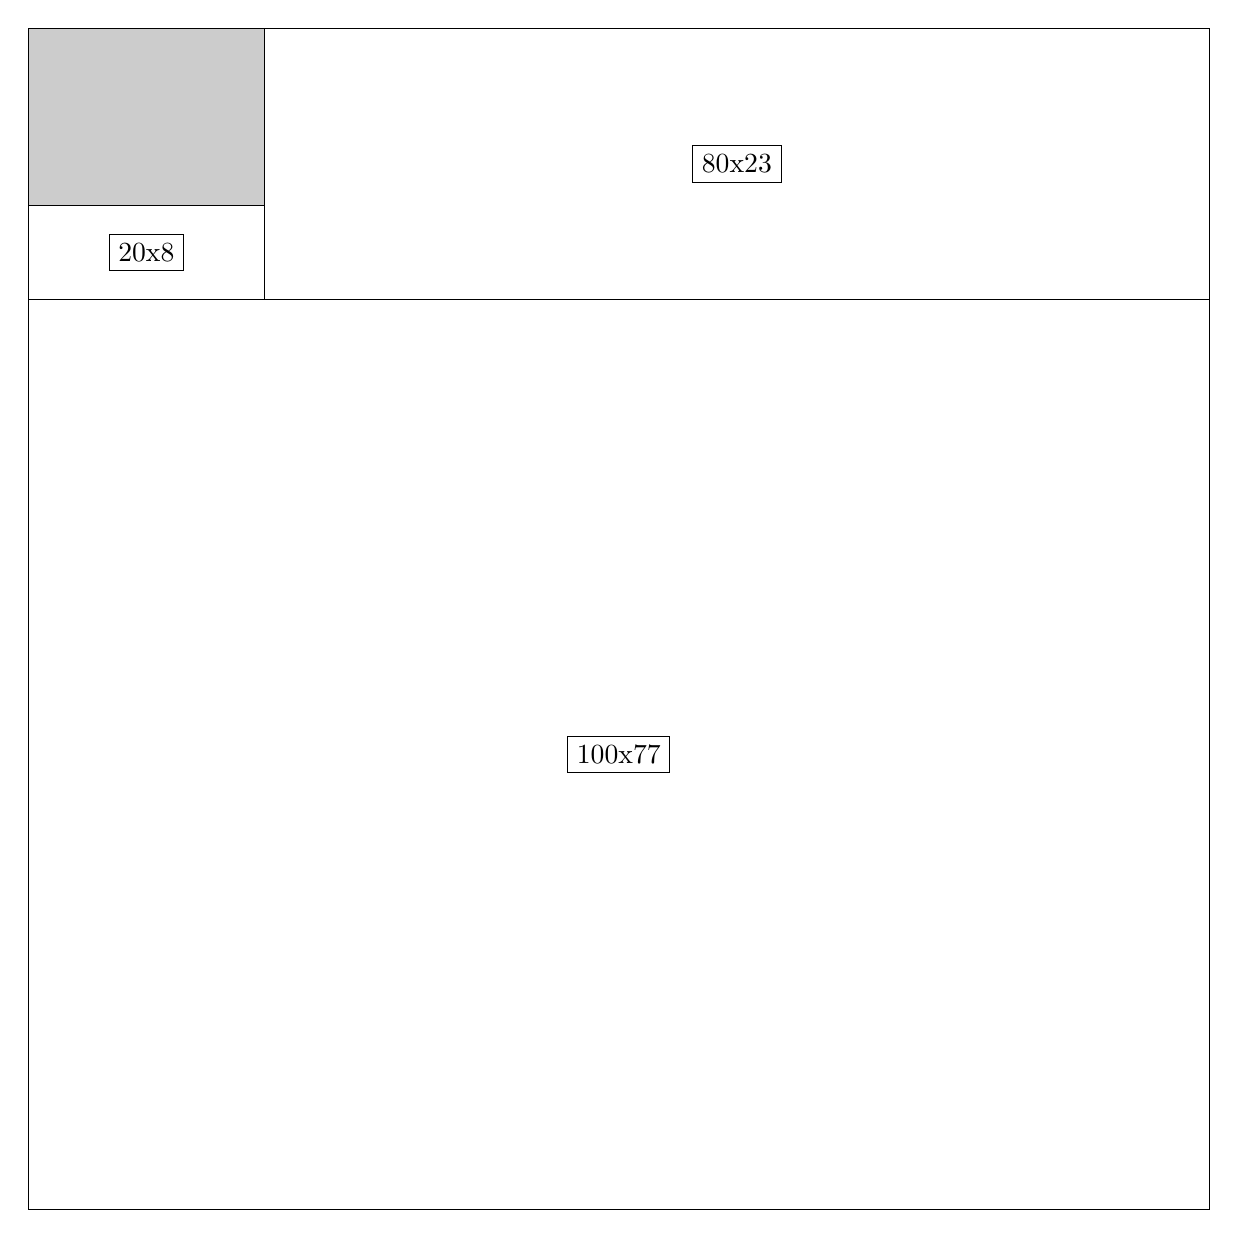
\begin{tikzpicture}[shorten >=1pt,scale=1.0,every node/.style={scale=1.0},->]
\tikzstyle{vertex}=[circle,fill=black!25,minimum size=14pt,inner sep=0pt]
\filldraw[fill=gray!40!white, draw=black] (0,0) rectangle (15.0,15.0);
\foreach \name/\x/\y/\w/\h in {100x77/0.0/0.0/15.0/11.549999999999999,80x23/3.0/11.549999999999999/12.0/3.4499999999999997,20x8/0.0/11.549999999999999/3.0/1.2}
\filldraw[fill=white!40!white, draw=black] (\x,\y) rectangle node[draw] (\name) {\name} ++(\w,\h);
\end{tikzpicture}


w =100 , h =77 , x =0 , y =0 , v =7700
\par
w =80 , h =23 , x =20 , y =77 , v =1840
\par
w =20 , h =8 , x =0 , y =77 , v =160
\par
\newpage


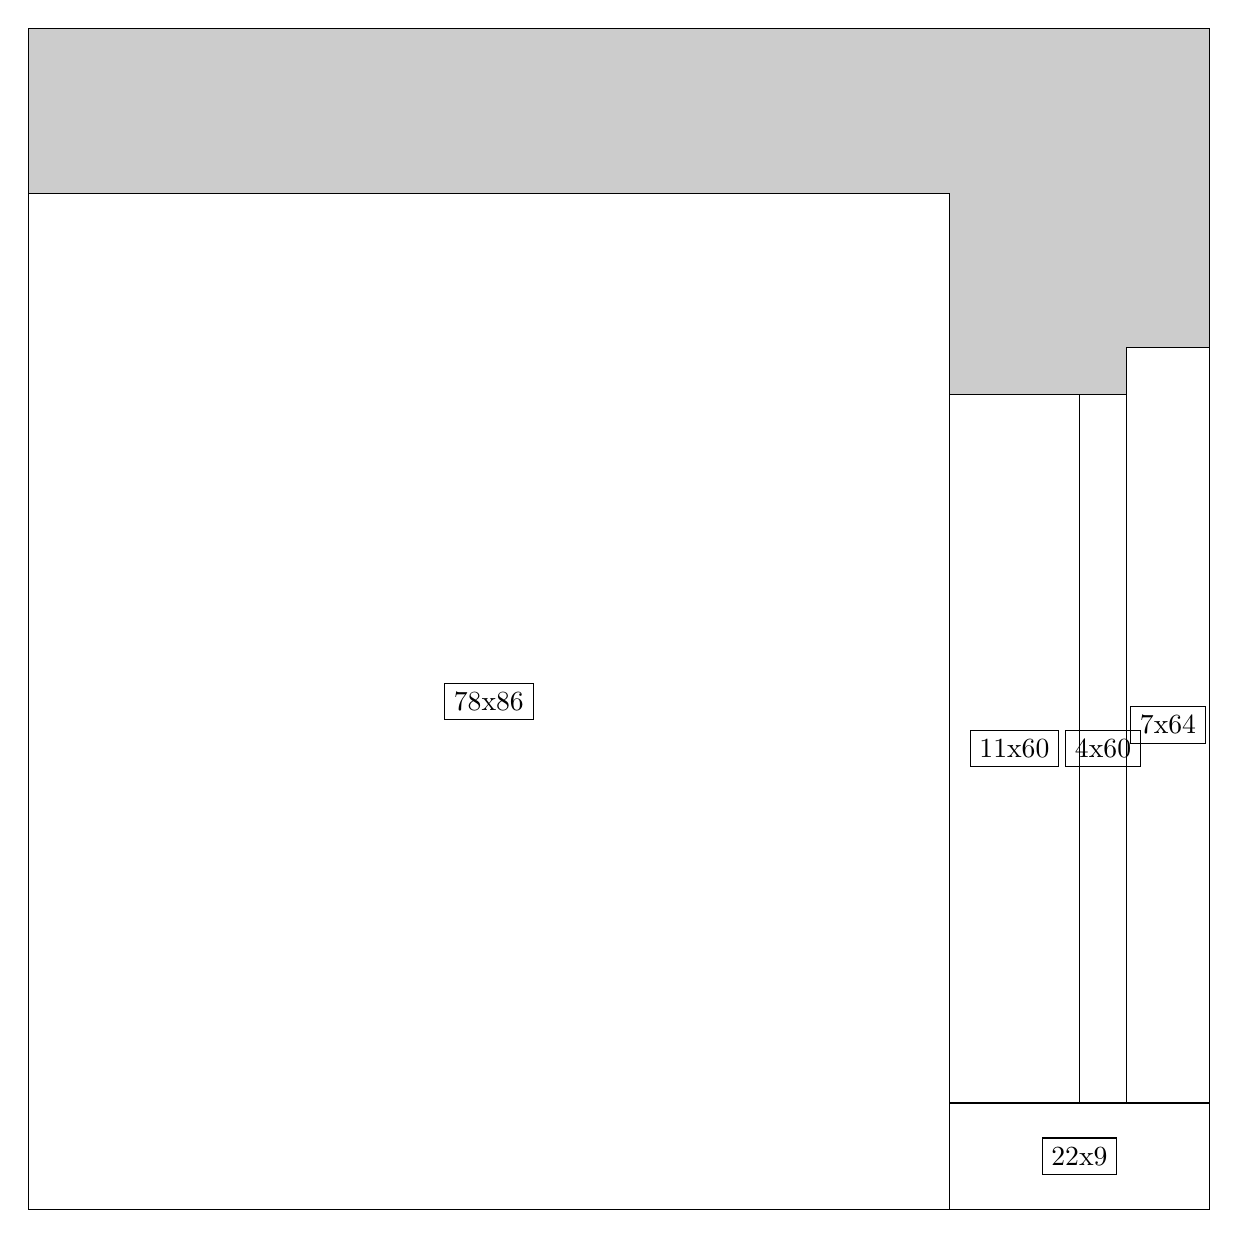
\begin{tikzpicture}[shorten >=1pt,scale=1.0,every node/.style={scale=1.0},->]
\tikzstyle{vertex}=[circle,fill=black!25,minimum size=14pt,inner sep=0pt]
\filldraw[fill=gray!40!white, draw=black] (0,0) rectangle (15.0,15.0);
\foreach \name/\x/\y/\w/\h in {78x86/0.0/0.0/11.7/12.9,11x60/11.7/1.3499999999999999/1.65/9.0,7x64/13.95/1.3499999999999999/1.05/9.6,4x60/13.35/1.3499999999999999/0.6/9.0,22x9/11.7/0.0/3.3/1.3499999999999999}
\filldraw[fill=white!40!white, draw=black] (\x,\y) rectangle node[draw] (\name) {\name} ++(\w,\h);
\end{tikzpicture}


w =78 , h =86 , x =0 , y =0 , v =6708
\par
w =11 , h =60 , x =78 , y =9 , v =660
\par
w =7 , h =64 , x =93 , y =9 , v =448
\par
w =4 , h =60 , x =89 , y =9 , v =240
\par
w =22 , h =9 , x =78 , y =0 , v =198
\par
\newpage


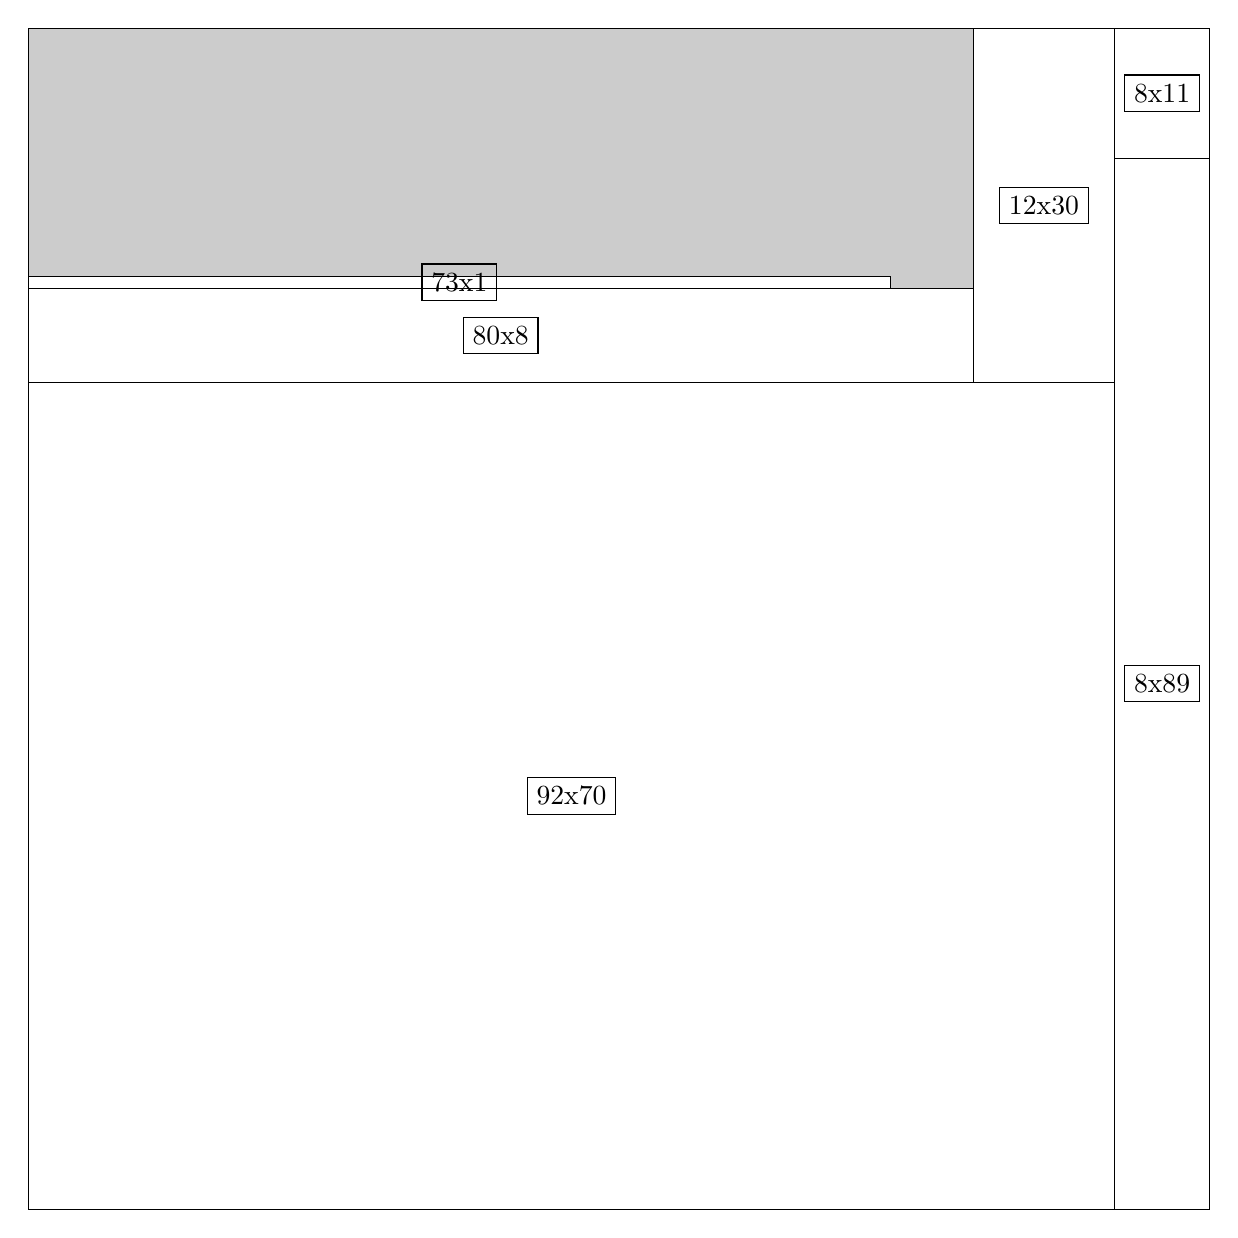
\begin{tikzpicture}[shorten >=1pt,scale=1.0,every node/.style={scale=1.0},->]
\tikzstyle{vertex}=[circle,fill=black!25,minimum size=14pt,inner sep=0pt]
\filldraw[fill=gray!40!white, draw=black] (0,0) rectangle (15.0,15.0);
\foreach \name/\x/\y/\w/\h in {92x70/0.0/0.0/13.799999999999999/10.5,8x89/13.799999999999999/0.0/1.2/13.35,80x8/0.0/10.5/12.0/1.2,12x30/12.0/10.5/1.7999999999999998/4.5,8x11/13.799999999999999/13.35/1.2/1.65,73x1/0.0/11.7/10.95/0.15}
\filldraw[fill=white!40!white, draw=black] (\x,\y) rectangle node[draw] (\name) {\name} ++(\w,\h);
\end{tikzpicture}


w =92 , h =70 , x =0 , y =0 , v =6440
\par
w =8 , h =89 , x =92 , y =0 , v =712
\par
w =80 , h =8 , x =0 , y =70 , v =640
\par
w =12 , h =30 , x =80 , y =70 , v =360
\par
w =8 , h =11 , x =92 , y =89 , v =88
\par
w =73 , h =1 , x =0 , y =78 , v =73
\par
\newpage


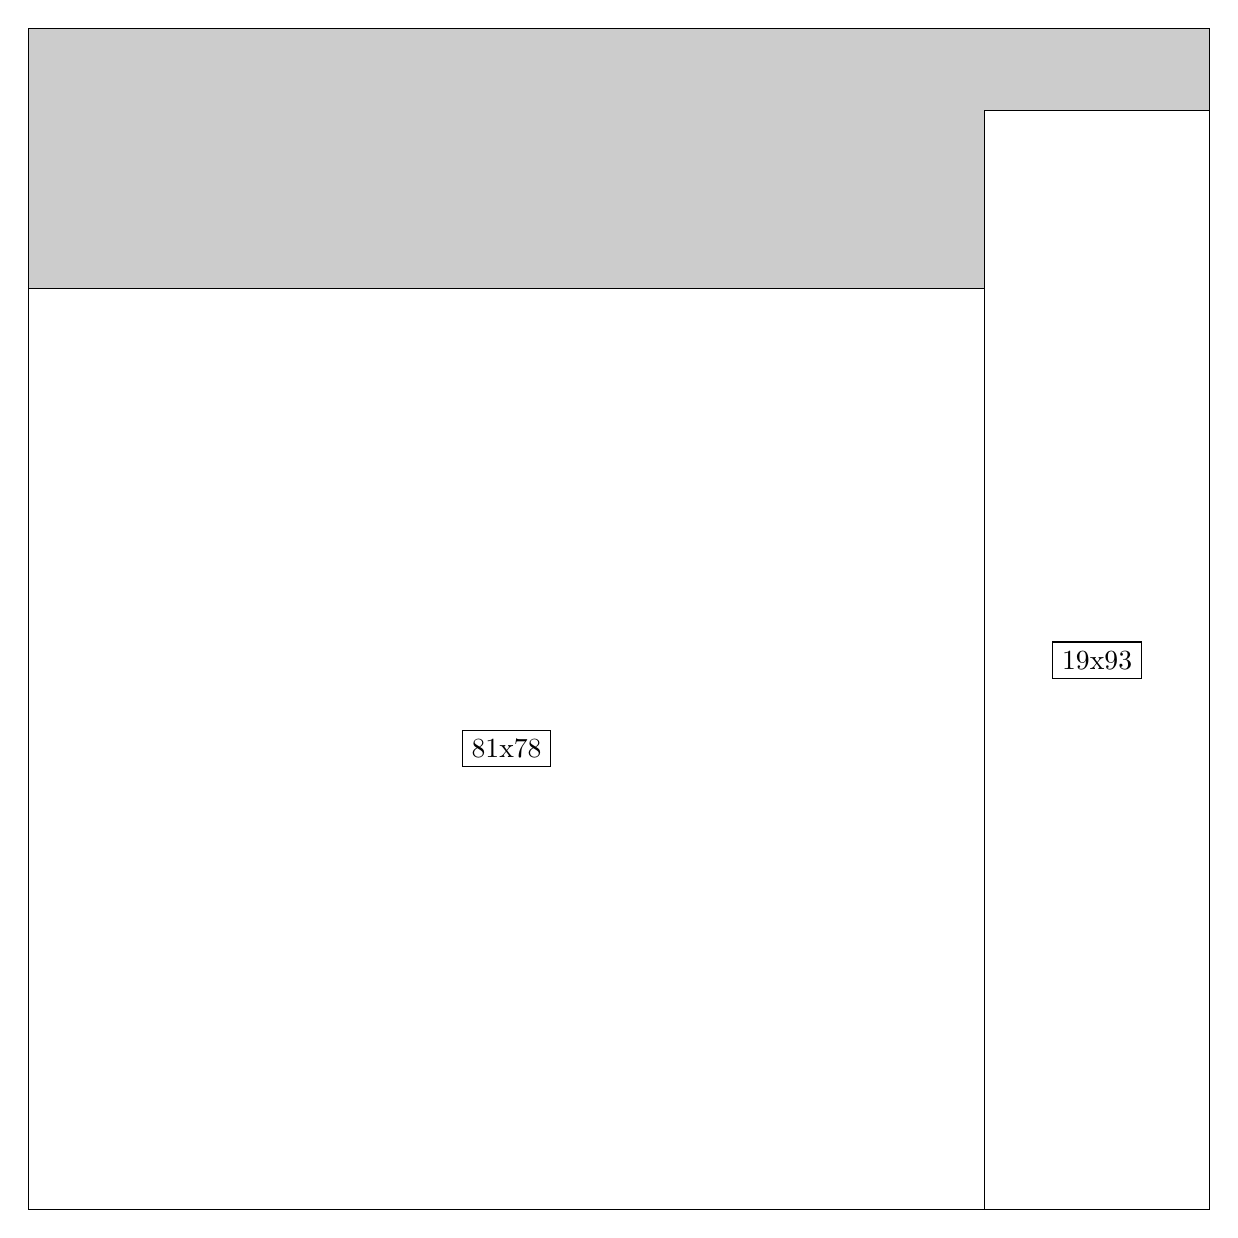
\begin{tikzpicture}[shorten >=1pt,scale=1.0,every node/.style={scale=1.0},->]
\tikzstyle{vertex}=[circle,fill=black!25,minimum size=14pt,inner sep=0pt]
\filldraw[fill=gray!40!white, draw=black] (0,0) rectangle (15.0,15.0);
\foreach \name/\x/\y/\w/\h in {81x78/0.0/0.0/12.15/11.7,19x93/12.15/0.0/2.85/13.95}
\filldraw[fill=white!40!white, draw=black] (\x,\y) rectangle node[draw] (\name) {\name} ++(\w,\h);
\end{tikzpicture}


w =81 , h =78 , x =0 , y =0 , v =6318
\par
w =19 , h =93 , x =81 , y =0 , v =1767
\par
\newpage


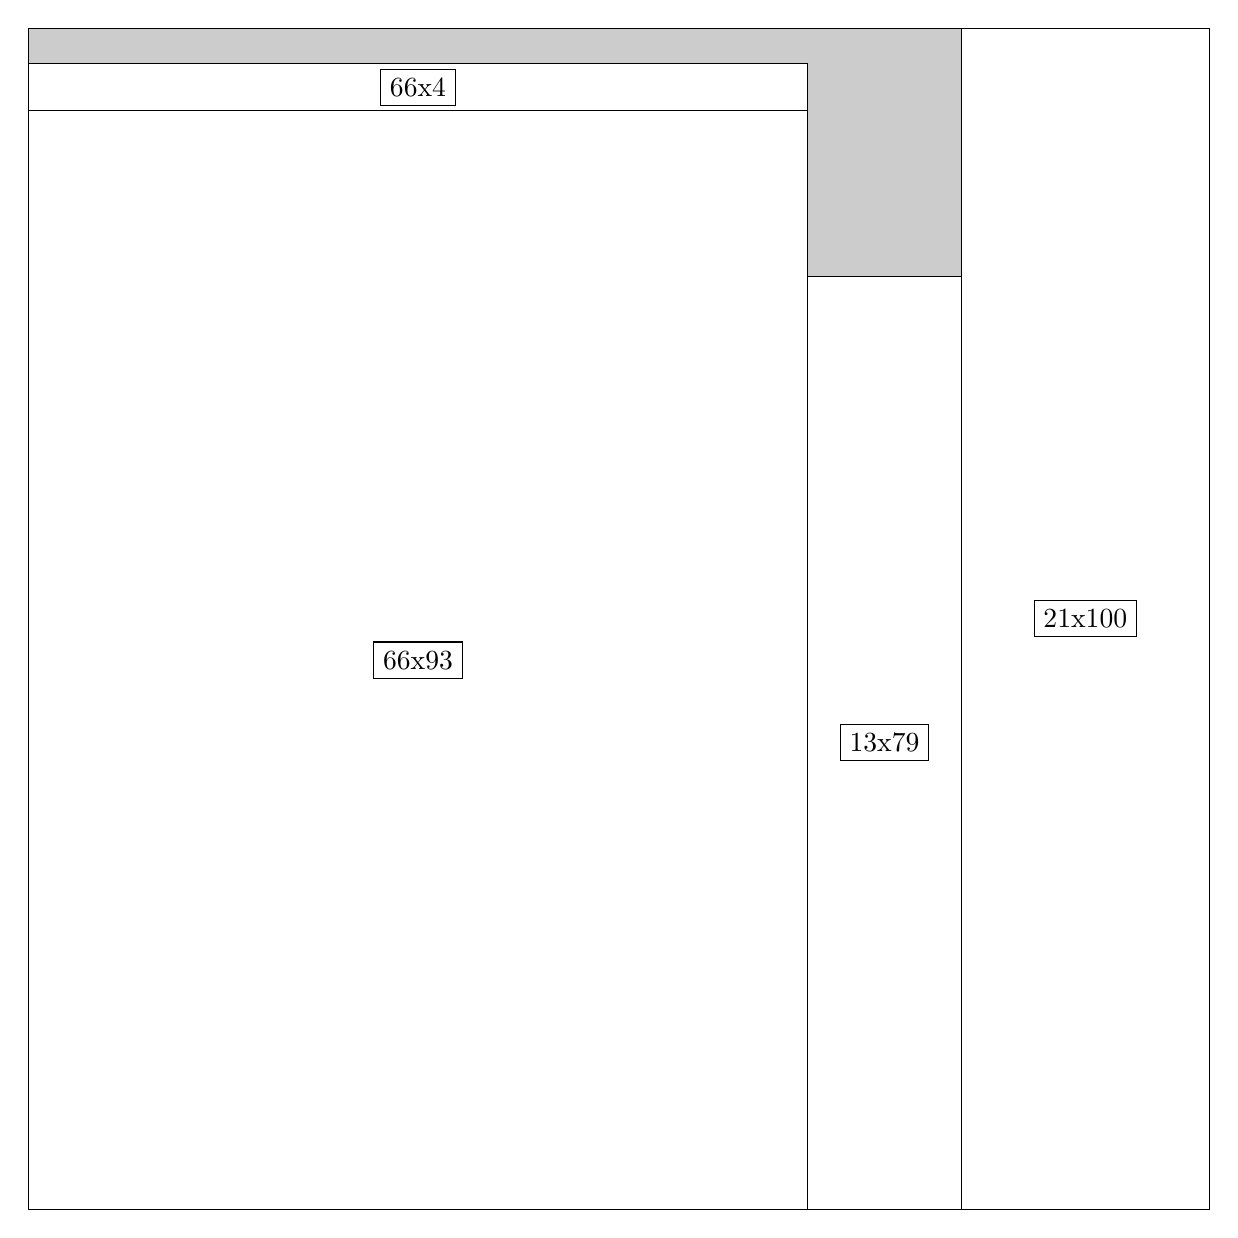
\begin{tikzpicture}[shorten >=1pt,scale=1.0,every node/.style={scale=1.0},->]
\tikzstyle{vertex}=[circle,fill=black!25,minimum size=14pt,inner sep=0pt]
\filldraw[fill=gray!40!white, draw=black] (0,0) rectangle (15.0,15.0);
\foreach \name/\x/\y/\w/\h in {66x93/0.0/0.0/9.9/13.95,21x100/11.85/0.0/3.15/15.0,13x79/9.9/0.0/1.95/11.85,66x4/0.0/13.95/9.9/0.6}
\filldraw[fill=white!40!white, draw=black] (\x,\y) rectangle node[draw] (\name) {\name} ++(\w,\h);
\end{tikzpicture}


w =66 , h =93 , x =0 , y =0 , v =6138
\par
w =21 , h =100 , x =79 , y =0 , v =2100
\par
w =13 , h =79 , x =66 , y =0 , v =1027
\par
w =66 , h =4 , x =0 , y =93 , v =264
\par
\newpage


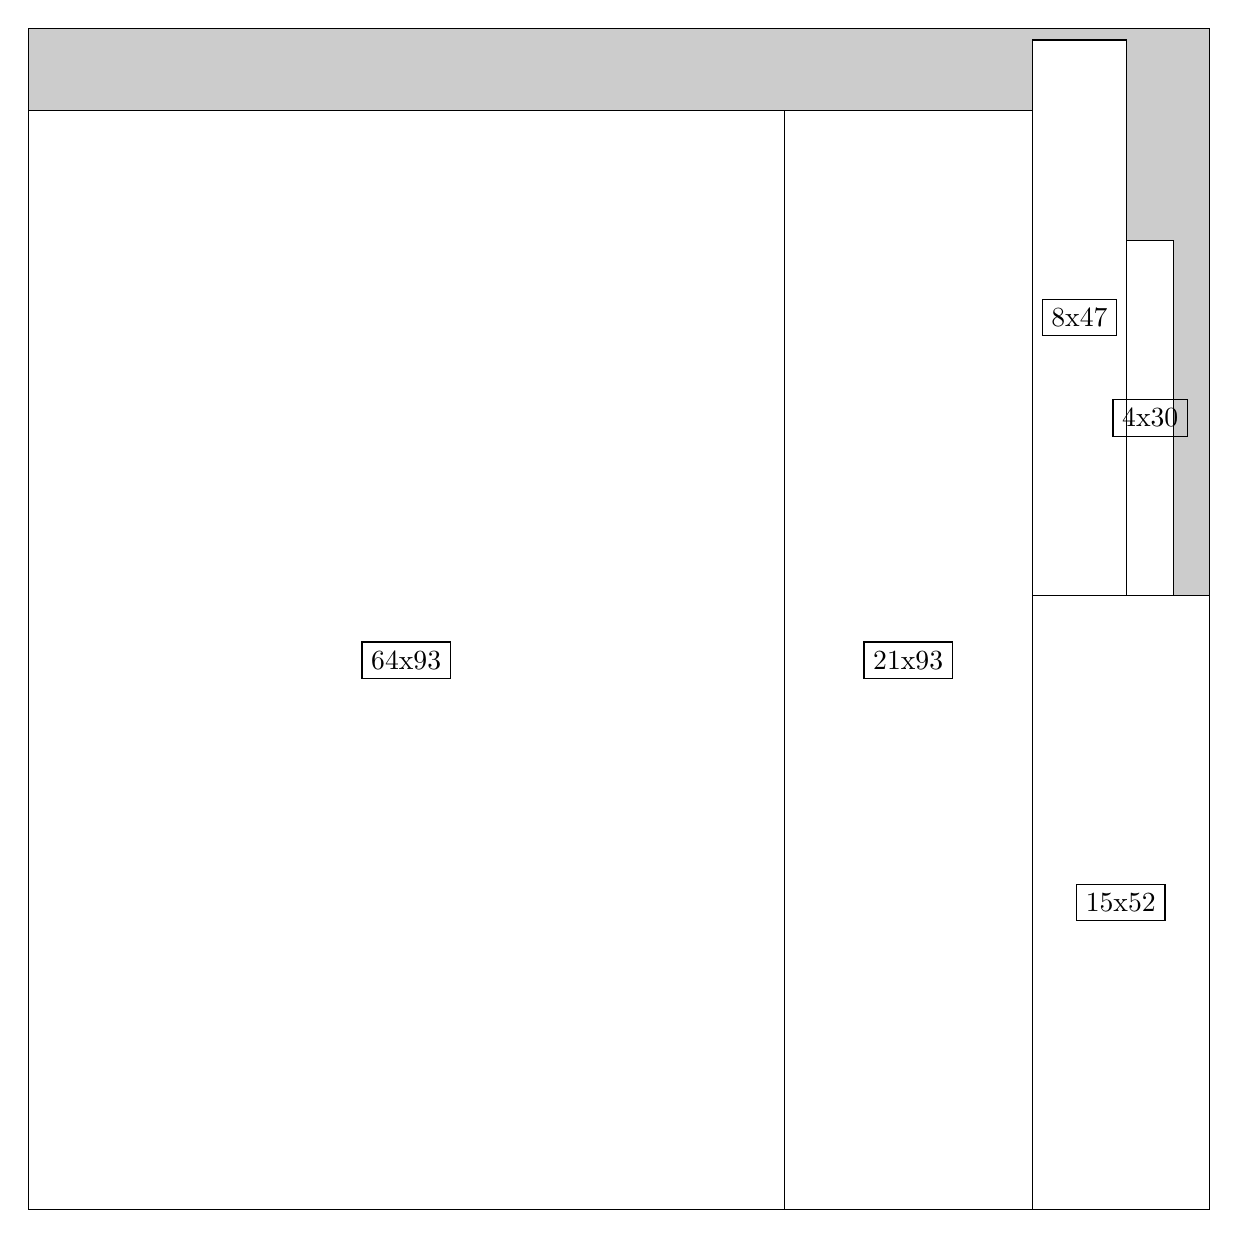
\begin{tikzpicture}[shorten >=1pt,scale=1.0,every node/.style={scale=1.0},->]
\tikzstyle{vertex}=[circle,fill=black!25,minimum size=14pt,inner sep=0pt]
\filldraw[fill=gray!40!white, draw=black] (0,0) rectangle (15.0,15.0);
\foreach \name/\x/\y/\w/\h in {64x93/0.0/0.0/9.6/13.95,21x93/9.6/0.0/3.15/13.95,15x52/12.75/0.0/2.25/7.8,8x47/12.75/7.8/1.2/7.05,4x30/13.95/7.8/0.6/4.5}
\filldraw[fill=white!40!white, draw=black] (\x,\y) rectangle node[draw] (\name) {\name} ++(\w,\h);
\end{tikzpicture}


w =64 , h =93 , x =0 , y =0 , v =5952
\par
w =21 , h =93 , x =64 , y =0 , v =1953
\par
w =15 , h =52 , x =85 , y =0 , v =780
\par
w =8 , h =47 , x =85 , y =52 , v =376
\par
w =4 , h =30 , x =93 , y =52 , v =120
\par
\newpage


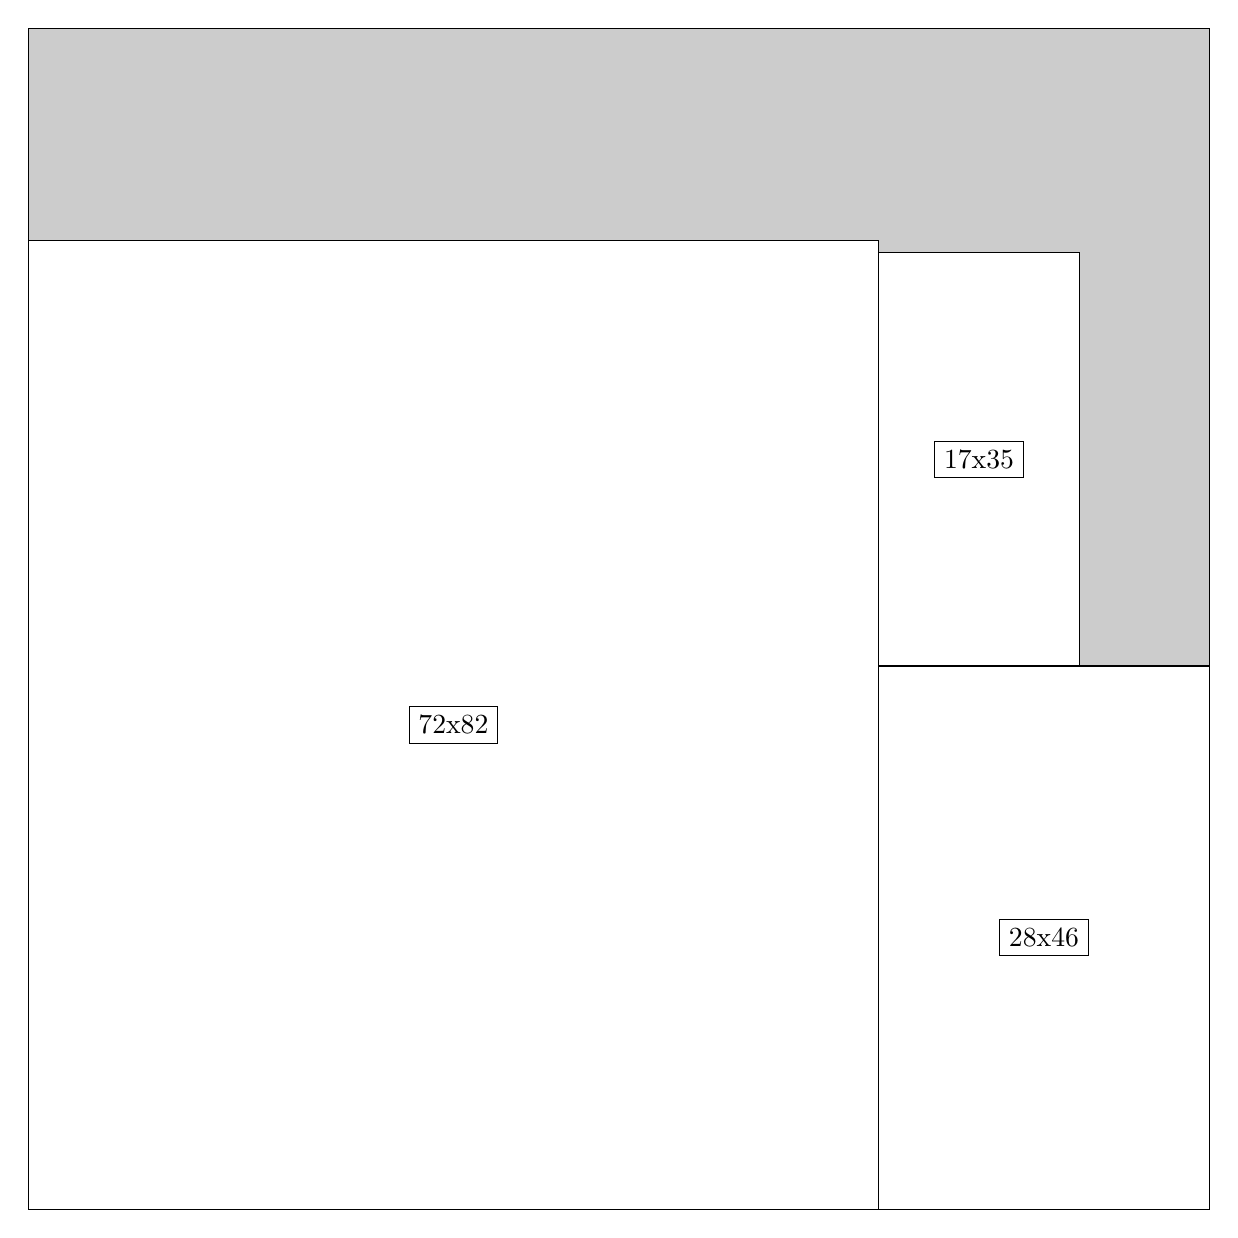
\begin{tikzpicture}[shorten >=1pt,scale=1.0,every node/.style={scale=1.0},->]
\tikzstyle{vertex}=[circle,fill=black!25,minimum size=14pt,inner sep=0pt]
\filldraw[fill=gray!40!white, draw=black] (0,0) rectangle (15.0,15.0);
\foreach \name/\x/\y/\w/\h in {72x82/0.0/0.0/10.799999999999999/12.299999999999999,28x46/10.799999999999999/0.0/4.2/6.8999999999999995,17x35/10.799999999999999/6.8999999999999995/2.55/5.25}
\filldraw[fill=white!40!white, draw=black] (\x,\y) rectangle node[draw] (\name) {\name} ++(\w,\h);
\end{tikzpicture}


w =72 , h =82 , x =0 , y =0 , v =5904
\par
w =28 , h =46 , x =72 , y =0 , v =1288
\par
w =17 , h =35 , x =72 , y =46 , v =595
\par
\newpage


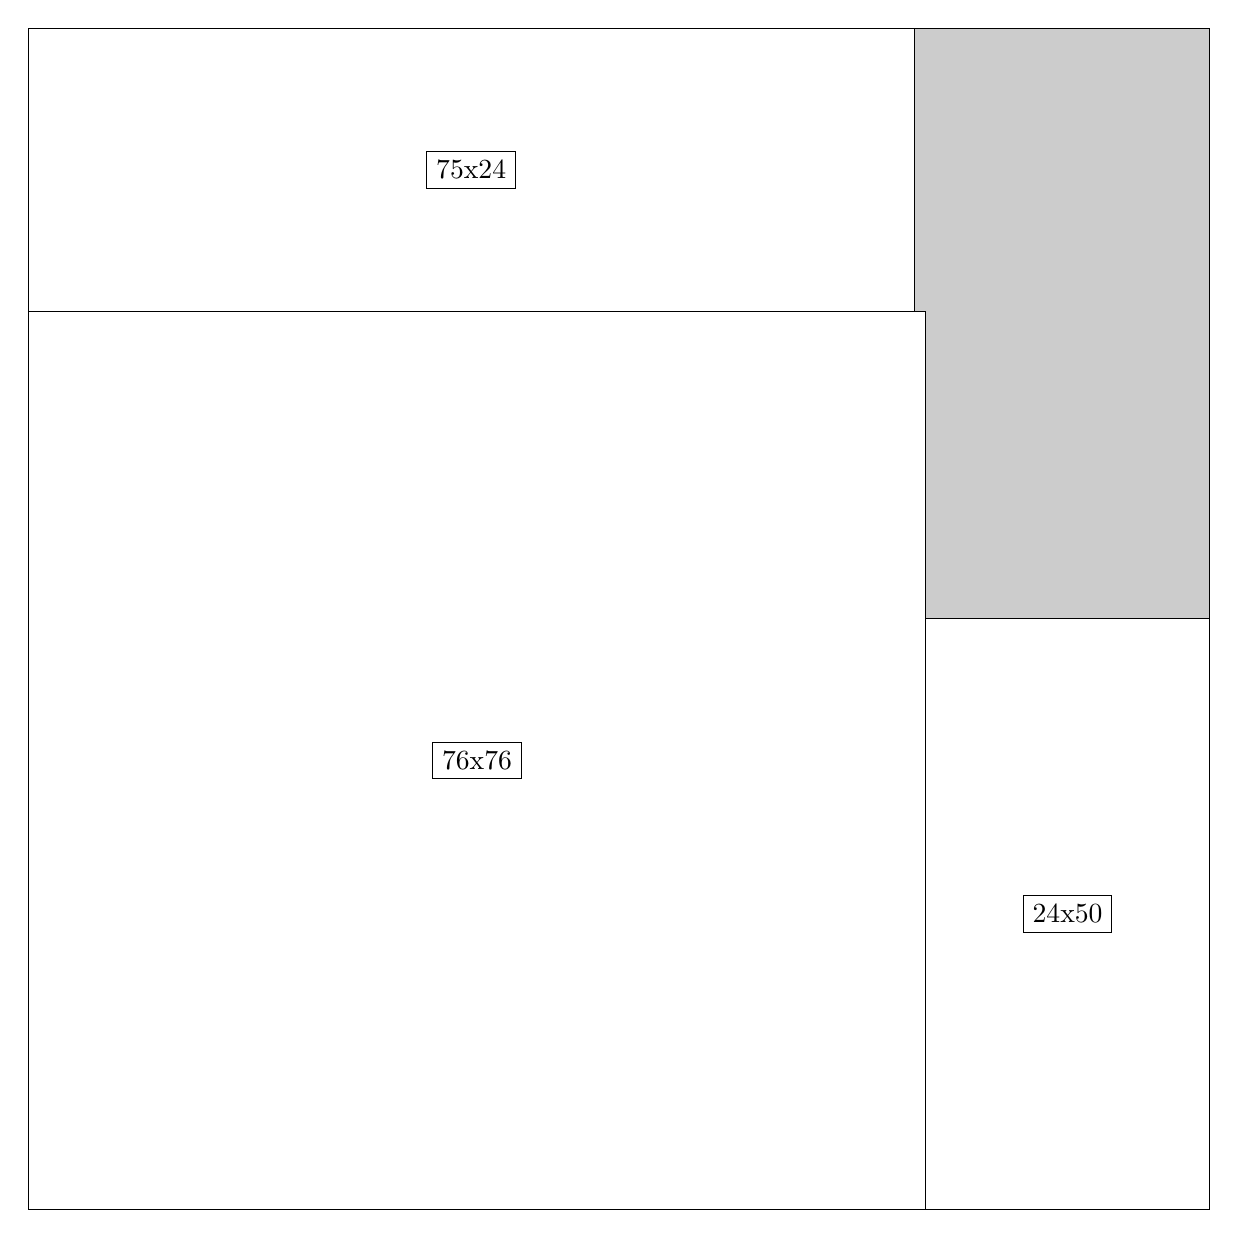
\begin{tikzpicture}[shorten >=1pt,scale=1.0,every node/.style={scale=1.0},->]
\tikzstyle{vertex}=[circle,fill=black!25,minimum size=14pt,inner sep=0pt]
\filldraw[fill=gray!40!white, draw=black] (0,0) rectangle (15.0,15.0);
\foreach \name/\x/\y/\w/\h in {76x76/0.0/0.0/11.4/11.4,75x24/0.0/11.4/11.25/3.5999999999999996,24x50/11.4/0.0/3.5999999999999996/7.5}
\filldraw[fill=white!40!white, draw=black] (\x,\y) rectangle node[draw] (\name) {\name} ++(\w,\h);
\end{tikzpicture}


w =76 , h =76 , x =0 , y =0 , v =5776
\par
w =75 , h =24 , x =0 , y =76 , v =1800
\par
w =24 , h =50 , x =76 , y =0 , v =1200
\par
\newpage


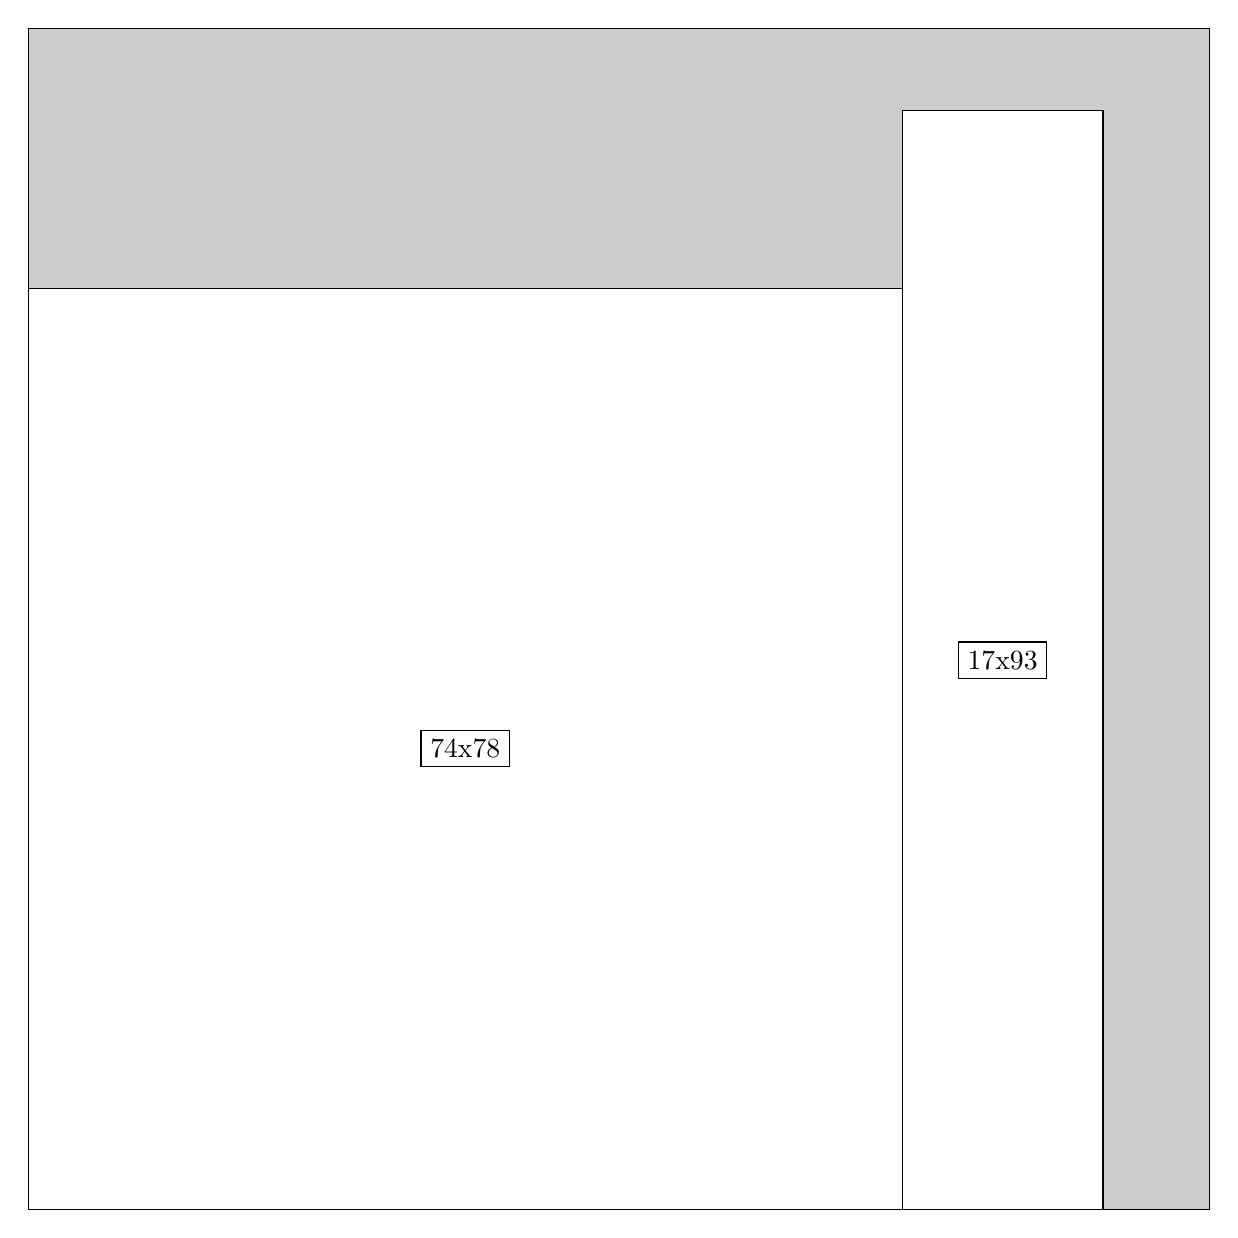
\begin{tikzpicture}[shorten >=1pt,scale=1.0,every node/.style={scale=1.0},->]
\tikzstyle{vertex}=[circle,fill=black!25,minimum size=14pt,inner sep=0pt]
\filldraw[fill=gray!40!white, draw=black] (0,0) rectangle (15.0,15.0);
\foreach \name/\x/\y/\w/\h in {74x78/0.0/0.0/11.1/11.7,17x93/11.1/0.0/2.55/13.95}
\filldraw[fill=white!40!white, draw=black] (\x,\y) rectangle node[draw] (\name) {\name} ++(\w,\h);
\end{tikzpicture}


w =74 , h =78 , x =0 , y =0 , v =5772
\par
w =17 , h =93 , x =74 , y =0 , v =1581
\par
\newpage


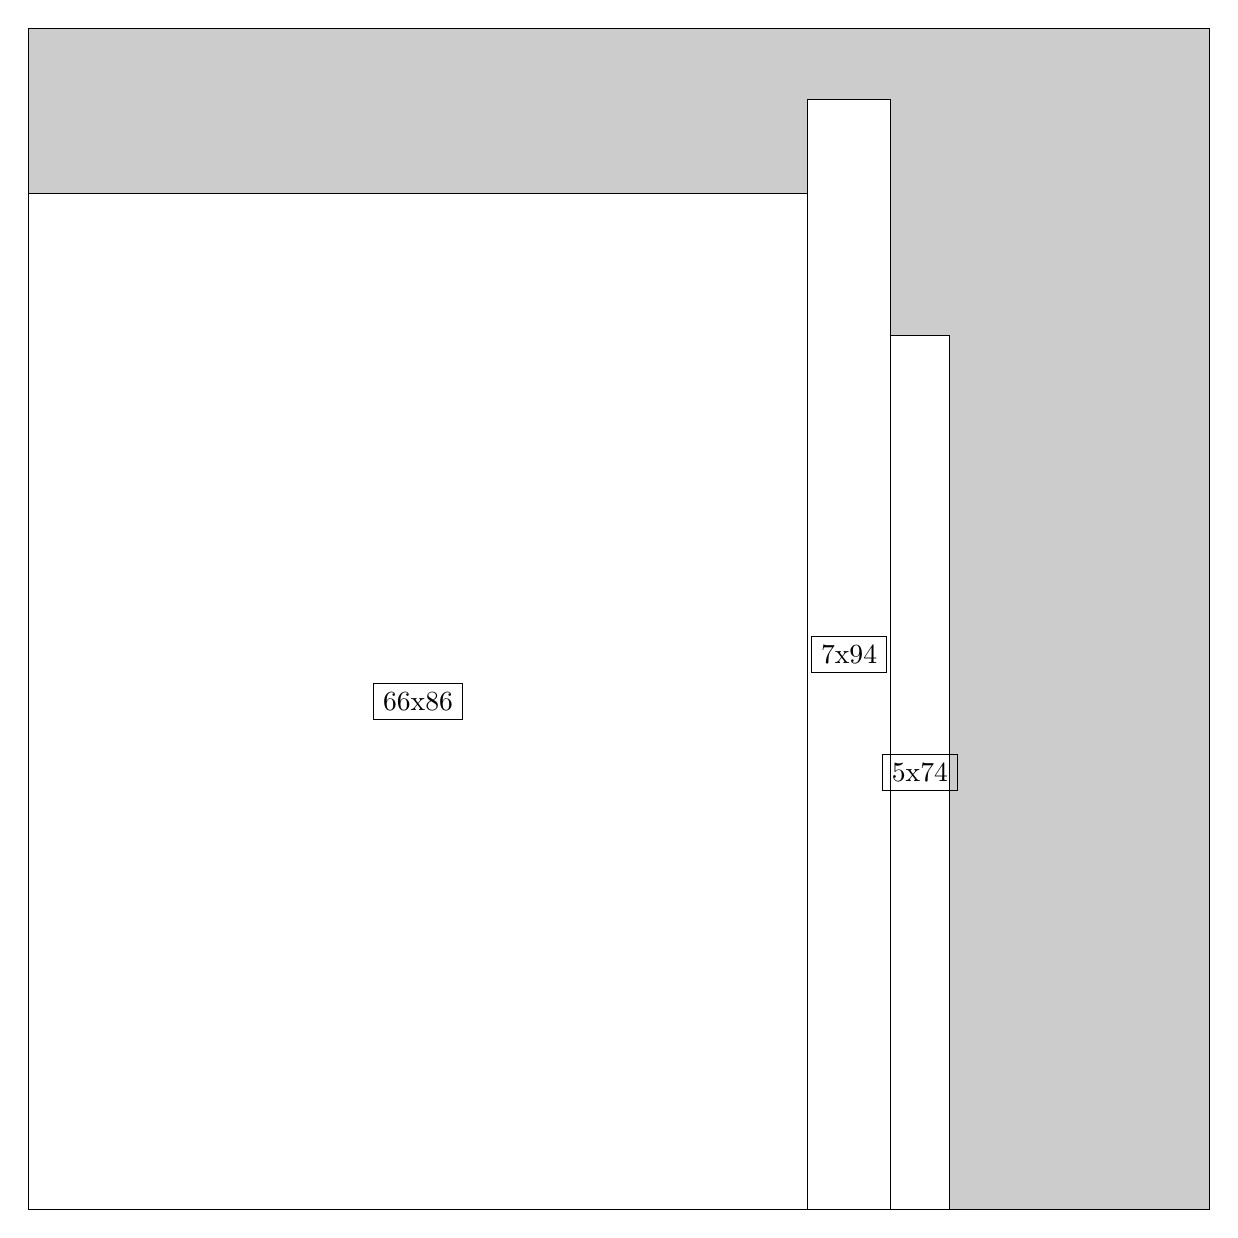
\begin{tikzpicture}[shorten >=1pt,scale=1.0,every node/.style={scale=1.0},->]
\tikzstyle{vertex}=[circle,fill=black!25,minimum size=14pt,inner sep=0pt]
\filldraw[fill=gray!40!white, draw=black] (0,0) rectangle (15.0,15.0);
\foreach \name/\x/\y/\w/\h in {66x86/0.0/0.0/9.9/12.9,7x94/9.9/0.0/1.05/14.1,5x74/10.95/0.0/0.75/11.1}
\filldraw[fill=white!40!white, draw=black] (\x,\y) rectangle node[draw] (\name) {\name} ++(\w,\h);
\end{tikzpicture}


w =66 , h =86 , x =0 , y =0 , v =5676
\par
w =7 , h =94 , x =66 , y =0 , v =658
\par
w =5 , h =74 , x =73 , y =0 , v =370
\par
\newpage


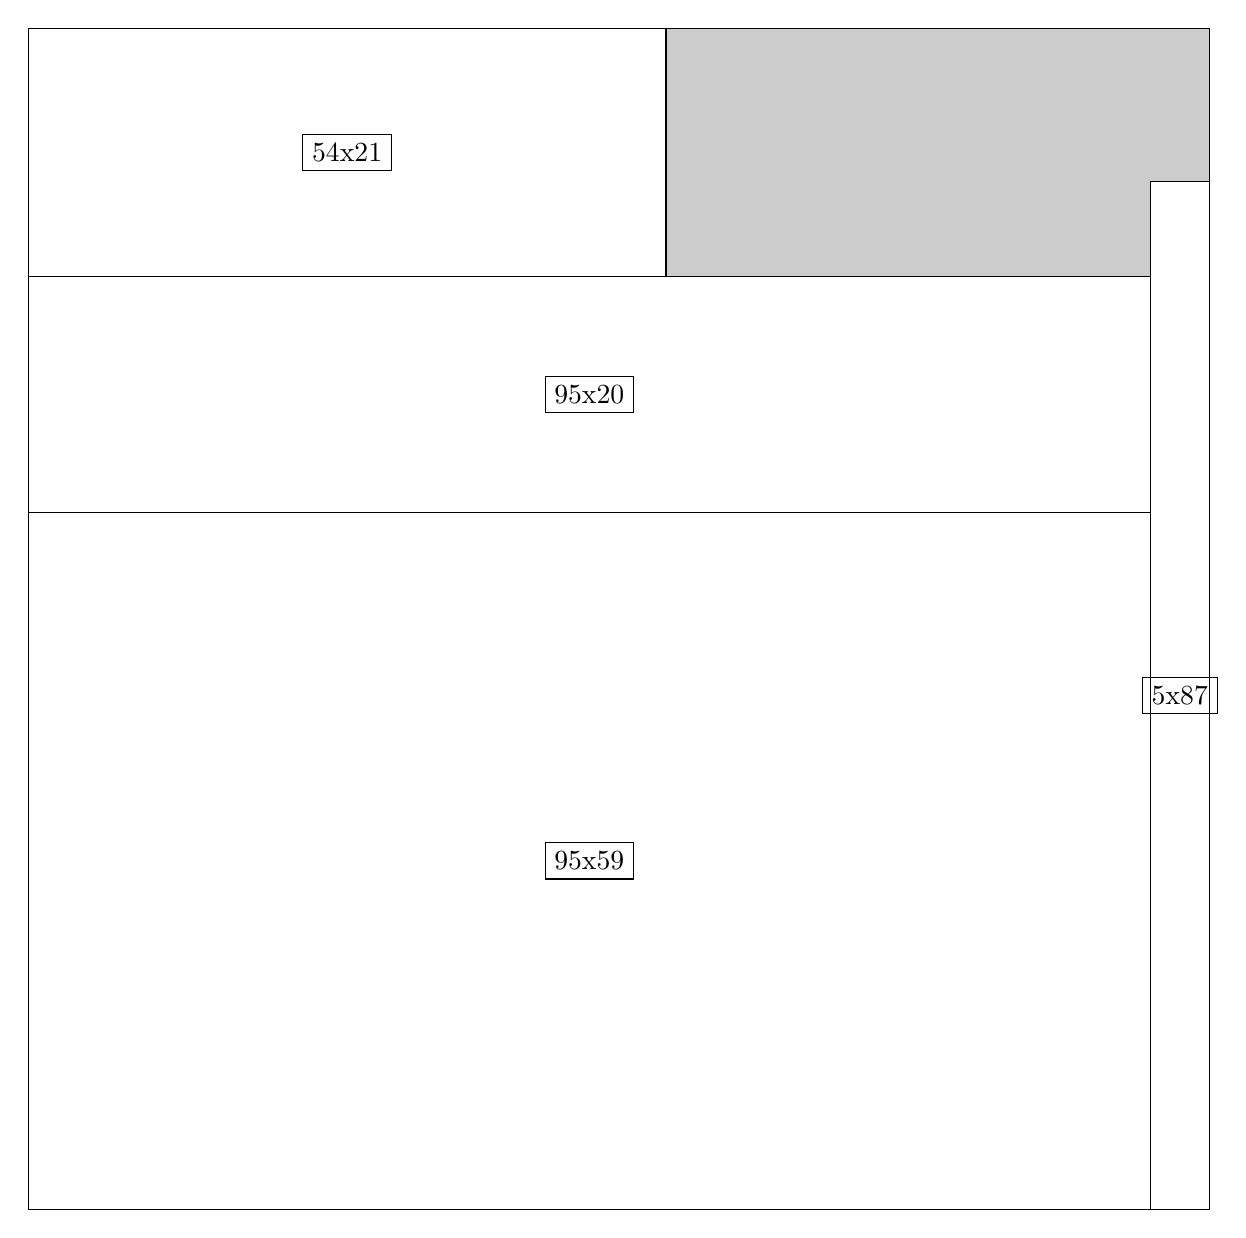
\begin{tikzpicture}[shorten >=1pt,scale=1.0,every node/.style={scale=1.0},->]
\tikzstyle{vertex}=[circle,fill=black!25,minimum size=14pt,inner sep=0pt]
\filldraw[fill=gray!40!white, draw=black] (0,0) rectangle (15.0,15.0);
\foreach \name/\x/\y/\w/\h in {95x59/0.0/0.0/14.25/8.85,95x20/0.0/8.85/14.25/3.0,54x21/0.0/11.85/8.1/3.15,5x87/14.25/0.0/0.75/13.049999999999999}
\filldraw[fill=white!40!white, draw=black] (\x,\y) rectangle node[draw] (\name) {\name} ++(\w,\h);
\end{tikzpicture}


w =95 , h =59 , x =0 , y =0 , v =5605
\par
w =95 , h =20 , x =0 , y =59 , v =1900
\par
w =54 , h =21 , x =0 , y =79 , v =1134
\par
w =5 , h =87 , x =95 , y =0 , v =435
\par
\newpage


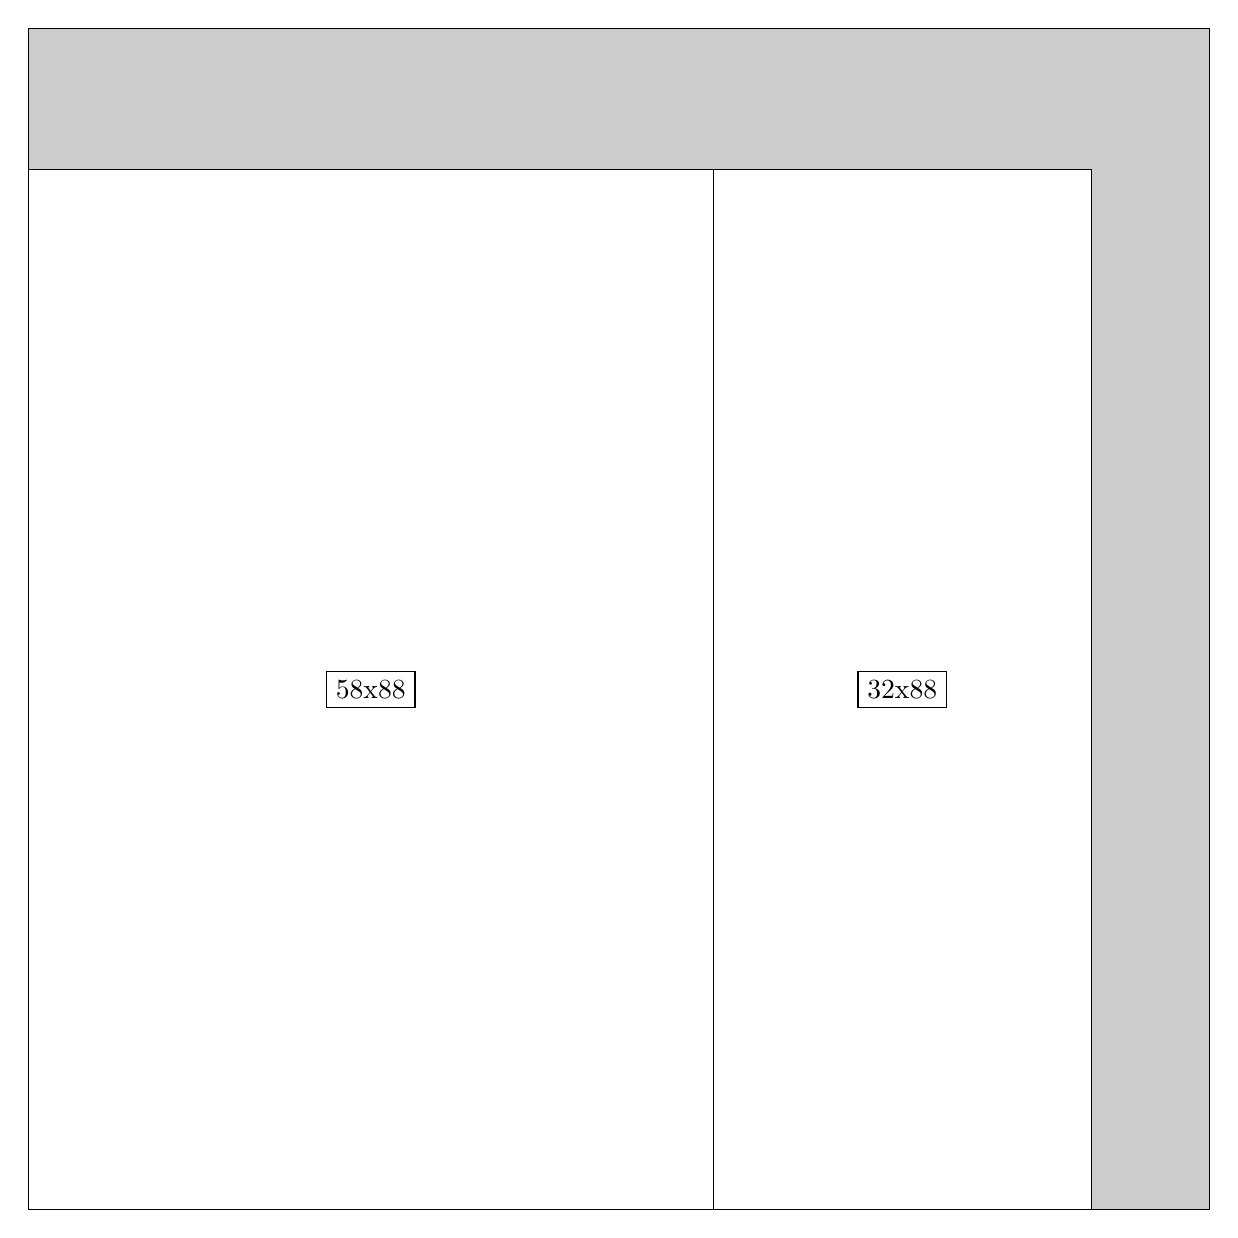
\begin{tikzpicture}[shorten >=1pt,scale=1.0,every node/.style={scale=1.0},->]
\tikzstyle{vertex}=[circle,fill=black!25,minimum size=14pt,inner sep=0pt]
\filldraw[fill=gray!40!white, draw=black] (0,0) rectangle (15.0,15.0);
\foreach \name/\x/\y/\w/\h in {58x88/0.0/0.0/8.7/13.2,32x88/8.7/0.0/4.8/13.2}
\filldraw[fill=white!40!white, draw=black] (\x,\y) rectangle node[draw] (\name) {\name} ++(\w,\h);
\end{tikzpicture}


w =58 , h =88 , x =0 , y =0 , v =5104
\par
w =32 , h =88 , x =58 , y =0 , v =2816
\par
\newpage


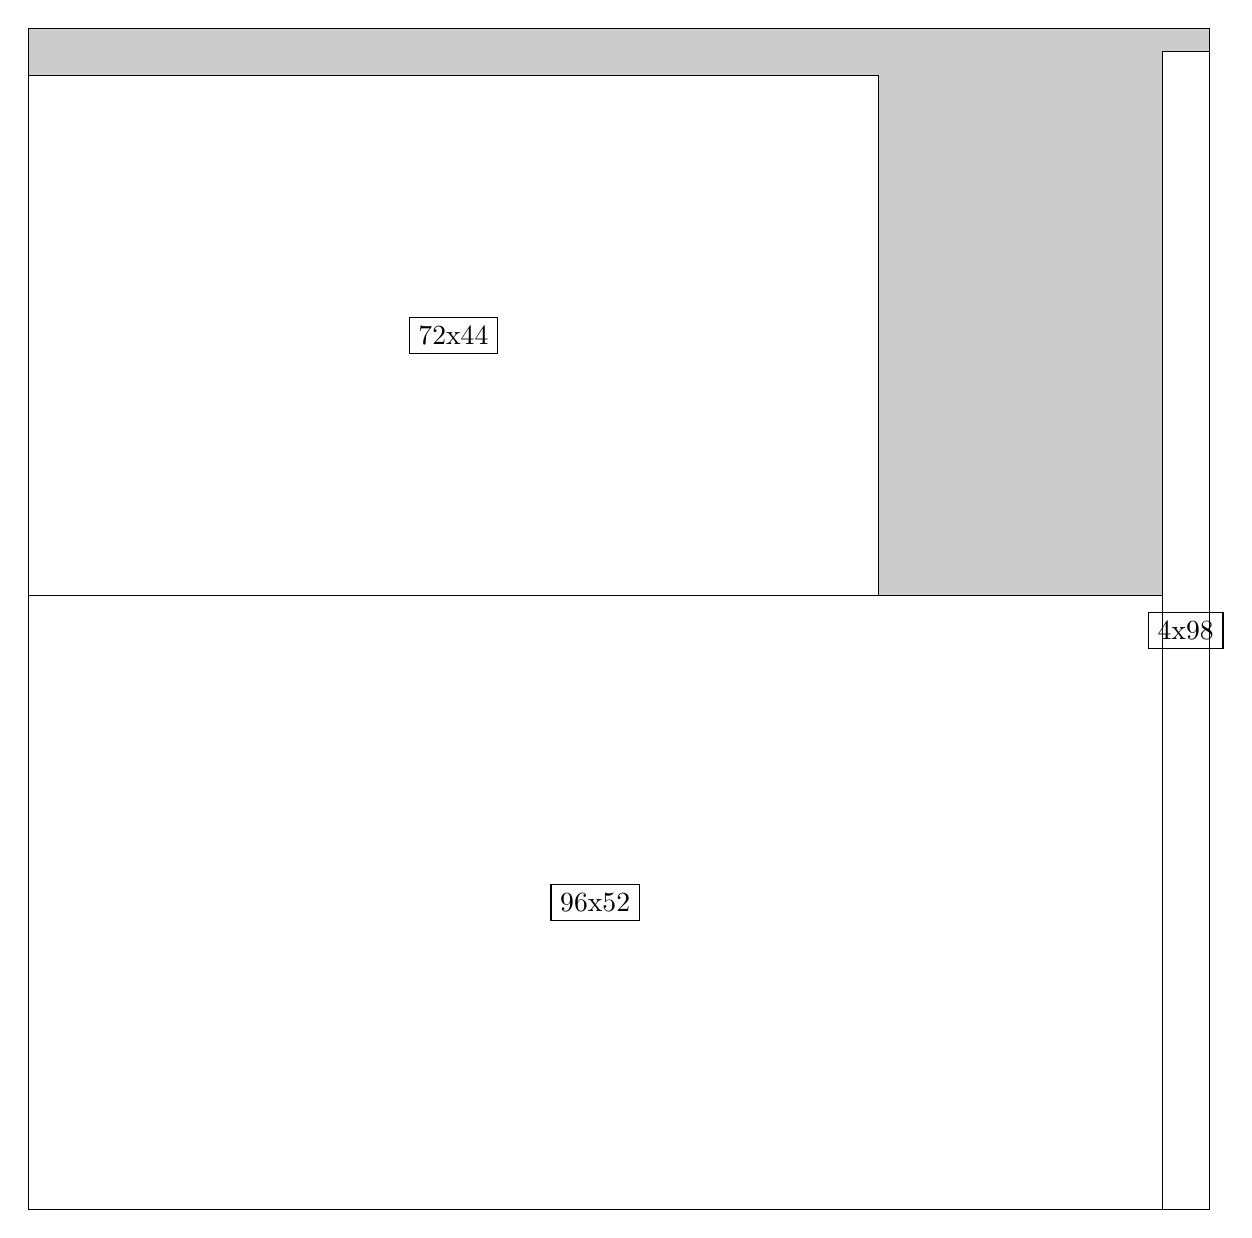
\begin{tikzpicture}[shorten >=1pt,scale=1.0,every node/.style={scale=1.0},->]
\tikzstyle{vertex}=[circle,fill=black!25,minimum size=14pt,inner sep=0pt]
\filldraw[fill=gray!40!white, draw=black] (0,0) rectangle (15.0,15.0);
\foreach \name/\x/\y/\w/\h in {96x52/0.0/0.0/14.399999999999999/7.8,72x44/0.0/7.8/10.799999999999999/6.6,4x98/14.399999999999999/0.0/0.6/14.7}
\filldraw[fill=white!40!white, draw=black] (\x,\y) rectangle node[draw] (\name) {\name} ++(\w,\h);
\end{tikzpicture}


w =96 , h =52 , x =0 , y =0 , v =4992
\par
w =72 , h =44 , x =0 , y =52 , v =3168
\par
w =4 , h =98 , x =96 , y =0 , v =392
\par
\newpage


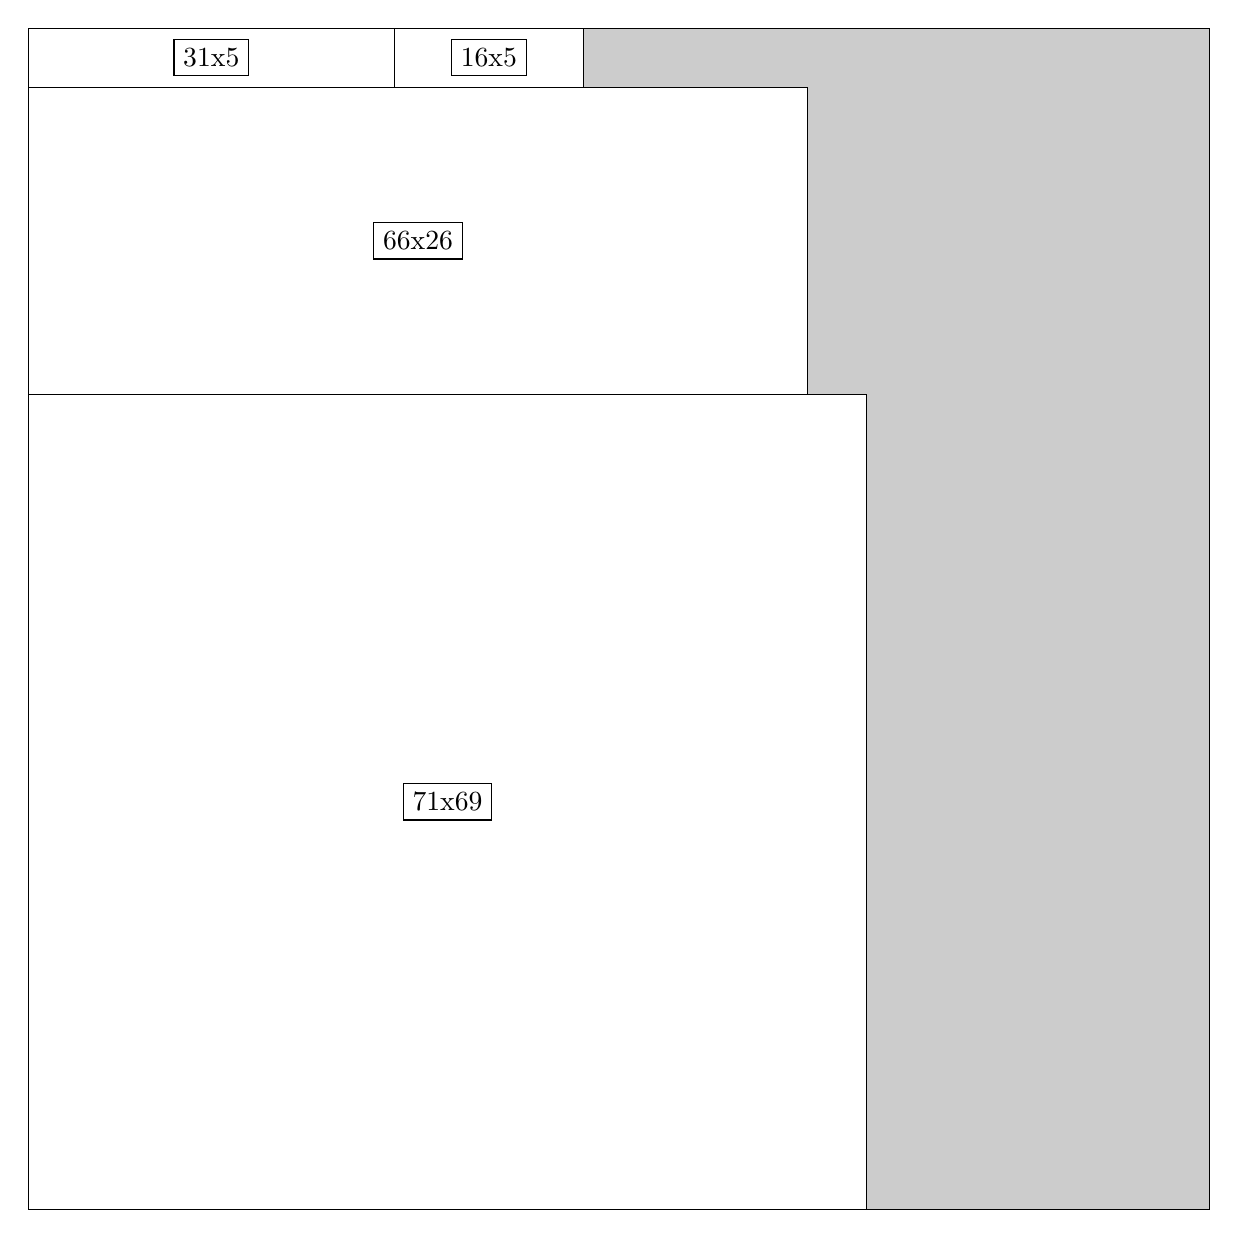
\begin{tikzpicture}[shorten >=1pt,scale=1.0,every node/.style={scale=1.0},->]
\tikzstyle{vertex}=[circle,fill=black!25,minimum size=14pt,inner sep=0pt]
\filldraw[fill=gray!40!white, draw=black] (0,0) rectangle (15.0,15.0);
\foreach \name/\x/\y/\w/\h in {71x69/0.0/0.0/10.65/10.35,66x26/0.0/10.35/9.9/3.9,31x5/0.0/14.25/4.6499999999999995/0.75,16x5/4.6499999999999995/14.25/2.4/0.75}
\filldraw[fill=white!40!white, draw=black] (\x,\y) rectangle node[draw] (\name) {\name} ++(\w,\h);
\end{tikzpicture}


w =71 , h =69 , x =0 , y =0 , v =4899
\par
w =66 , h =26 , x =0 , y =69 , v =1716
\par
w =31 , h =5 , x =0 , y =95 , v =155
\par
w =16 , h =5 , x =31 , y =95 , v =80
\par
\newpage


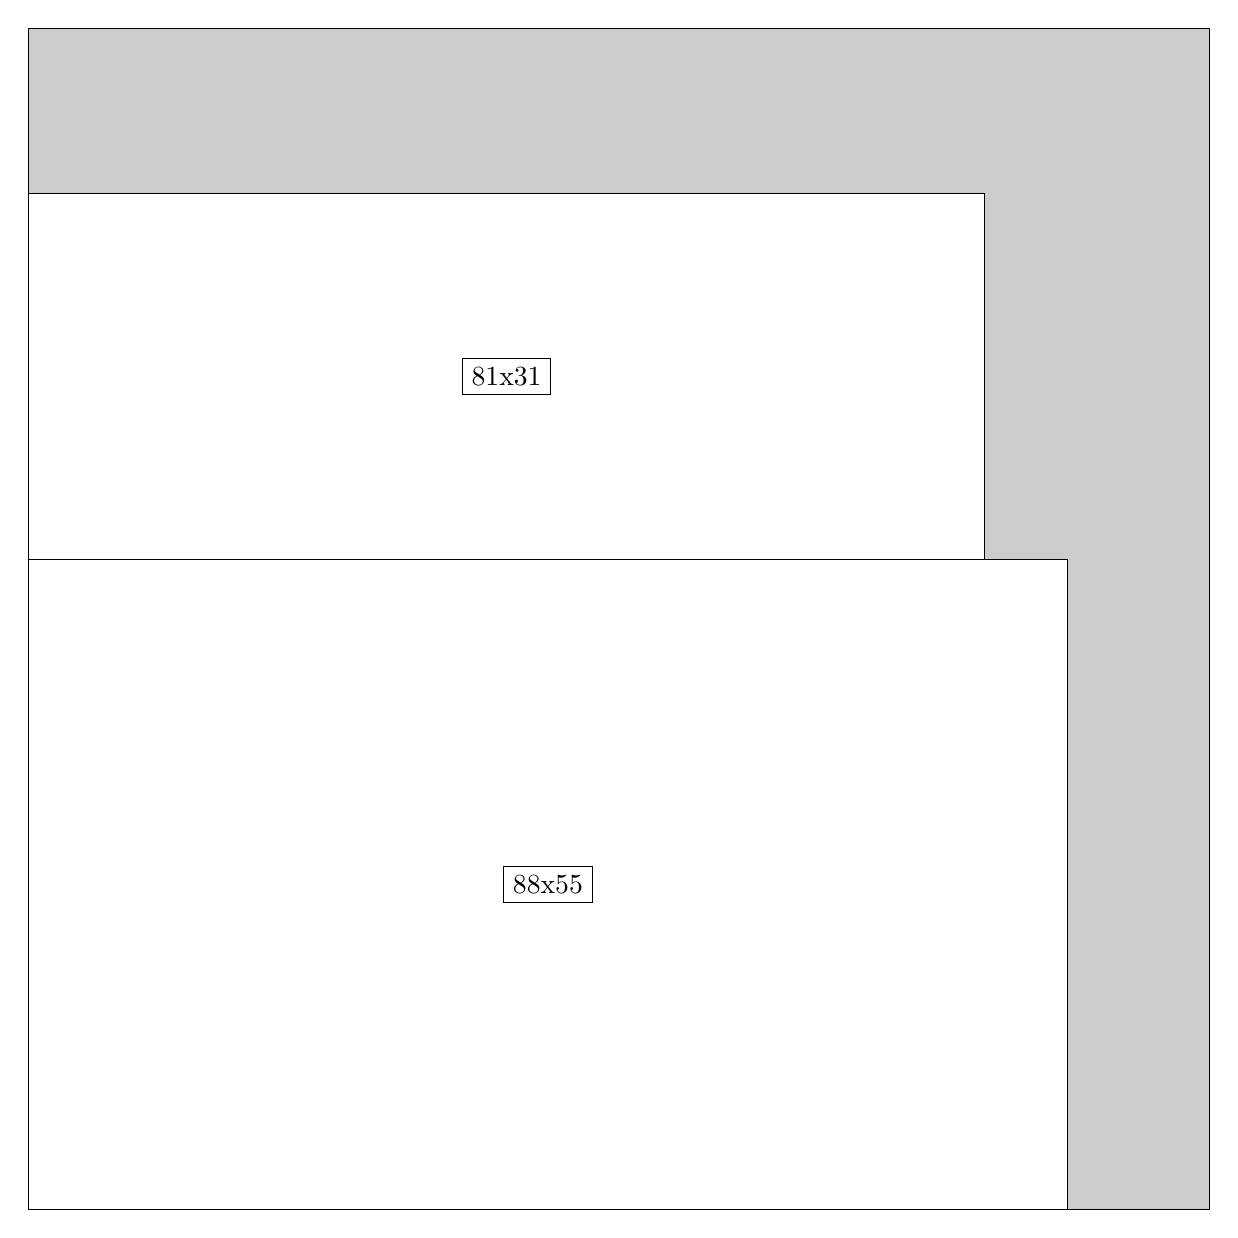
\begin{tikzpicture}[shorten >=1pt,scale=1.0,every node/.style={scale=1.0},->]
\tikzstyle{vertex}=[circle,fill=black!25,minimum size=14pt,inner sep=0pt]
\filldraw[fill=gray!40!white, draw=black] (0,0) rectangle (15.0,15.0);
\foreach \name/\x/\y/\w/\h in {88x55/0.0/0.0/13.2/8.25,81x31/0.0/8.25/12.15/4.6499999999999995}
\filldraw[fill=white!40!white, draw=black] (\x,\y) rectangle node[draw] (\name) {\name} ++(\w,\h);
\end{tikzpicture}


w =88 , h =55 , x =0 , y =0 , v =4840
\par
w =81 , h =31 , x =0 , y =55 , v =2511
\par
\newpage


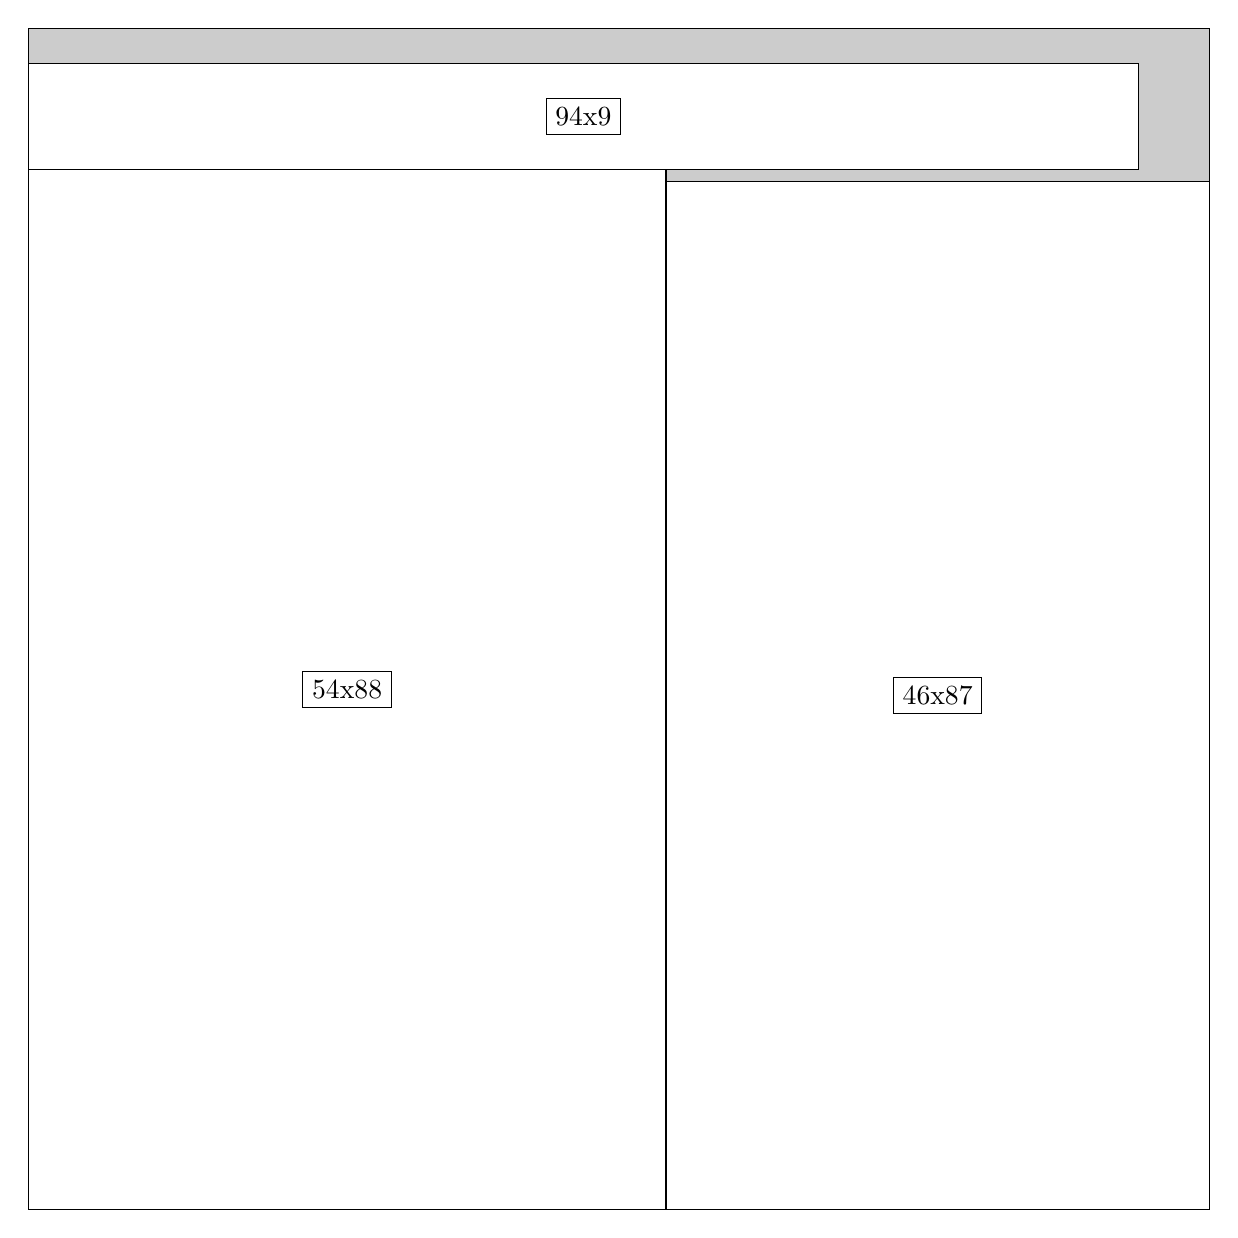
\begin{tikzpicture}[shorten >=1pt,scale=1.0,every node/.style={scale=1.0},->]
\tikzstyle{vertex}=[circle,fill=black!25,minimum size=14pt,inner sep=0pt]
\filldraw[fill=gray!40!white, draw=black] (0,0) rectangle (15.0,15.0);
\foreach \name/\x/\y/\w/\h in {54x88/0.0/0.0/8.1/13.2,46x87/8.1/0.0/6.8999999999999995/13.049999999999999,94x9/0.0/13.2/14.1/1.3499999999999999}
\filldraw[fill=white!40!white, draw=black] (\x,\y) rectangle node[draw] (\name) {\name} ++(\w,\h);
\end{tikzpicture}


w =54 , h =88 , x =0 , y =0 , v =4752
\par
w =46 , h =87 , x =54 , y =0 , v =4002
\par
w =94 , h =9 , x =0 , y =88 , v =846
\par
\newpage


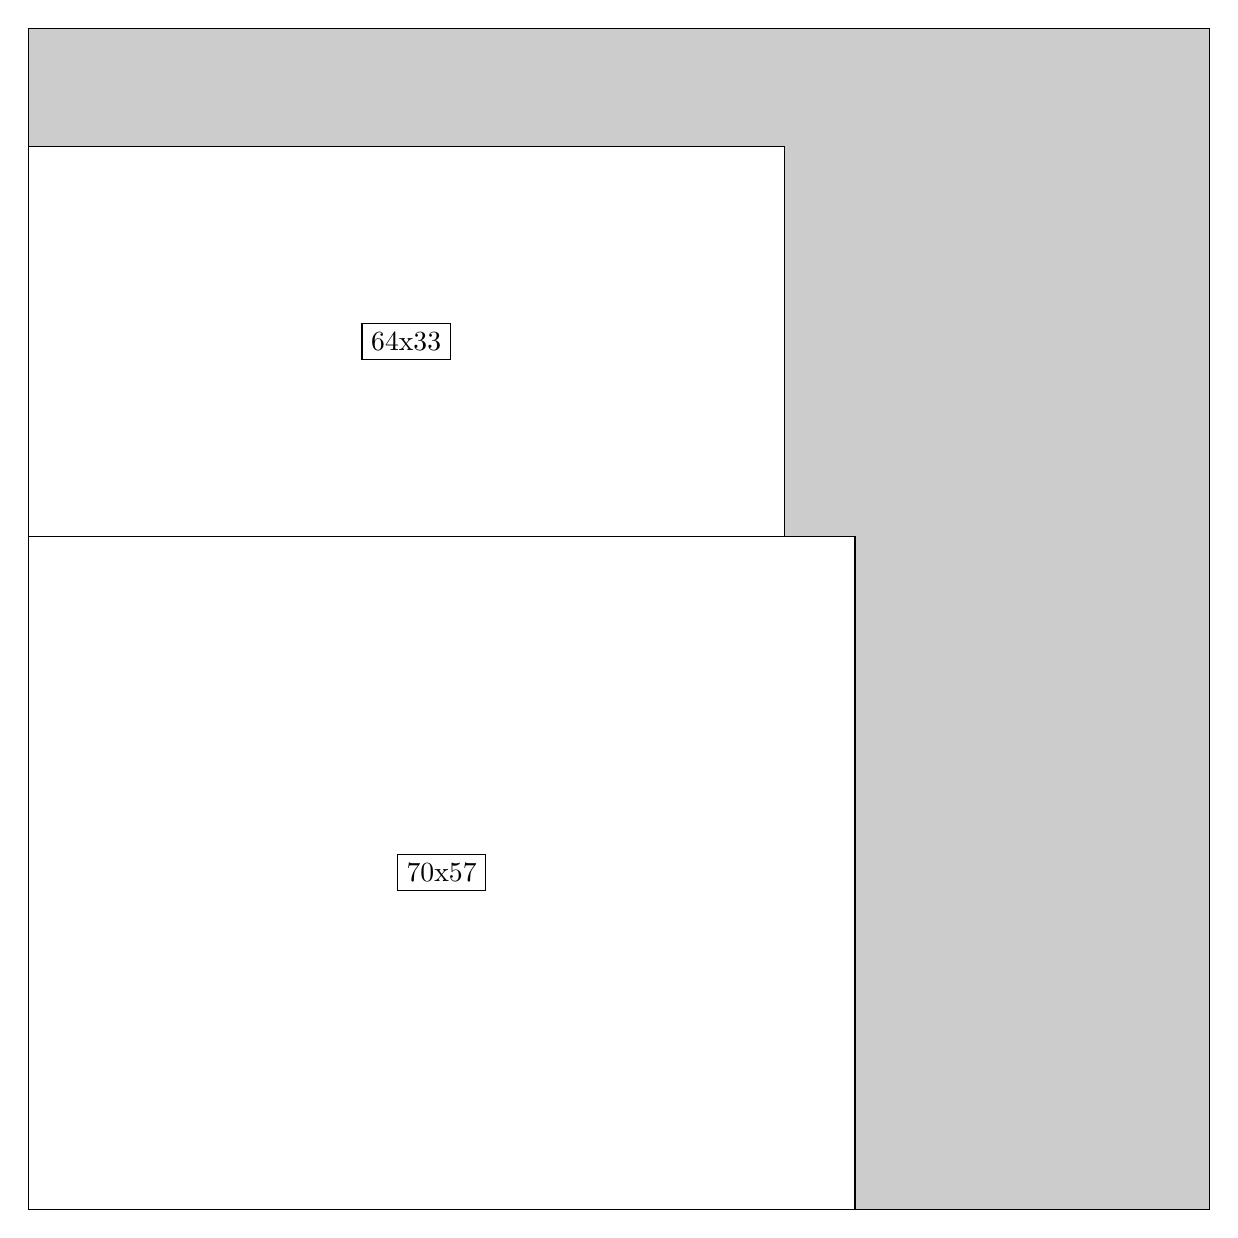
\begin{tikzpicture}[shorten >=1pt,scale=1.0,every node/.style={scale=1.0},->]
\tikzstyle{vertex}=[circle,fill=black!25,minimum size=14pt,inner sep=0pt]
\filldraw[fill=gray!40!white, draw=black] (0,0) rectangle (15.0,15.0);
\foreach \name/\x/\y/\w/\h in {70x57/0.0/0.0/10.5/8.549999999999999,64x33/0.0/8.549999999999999/9.6/4.95}
\filldraw[fill=white!40!white, draw=black] (\x,\y) rectangle node[draw] (\name) {\name} ++(\w,\h);
\end{tikzpicture}


w =70 , h =57 , x =0 , y =0 , v =3990
\par
w =64 , h =33 , x =0 , y =57 , v =2112
\par
\newpage


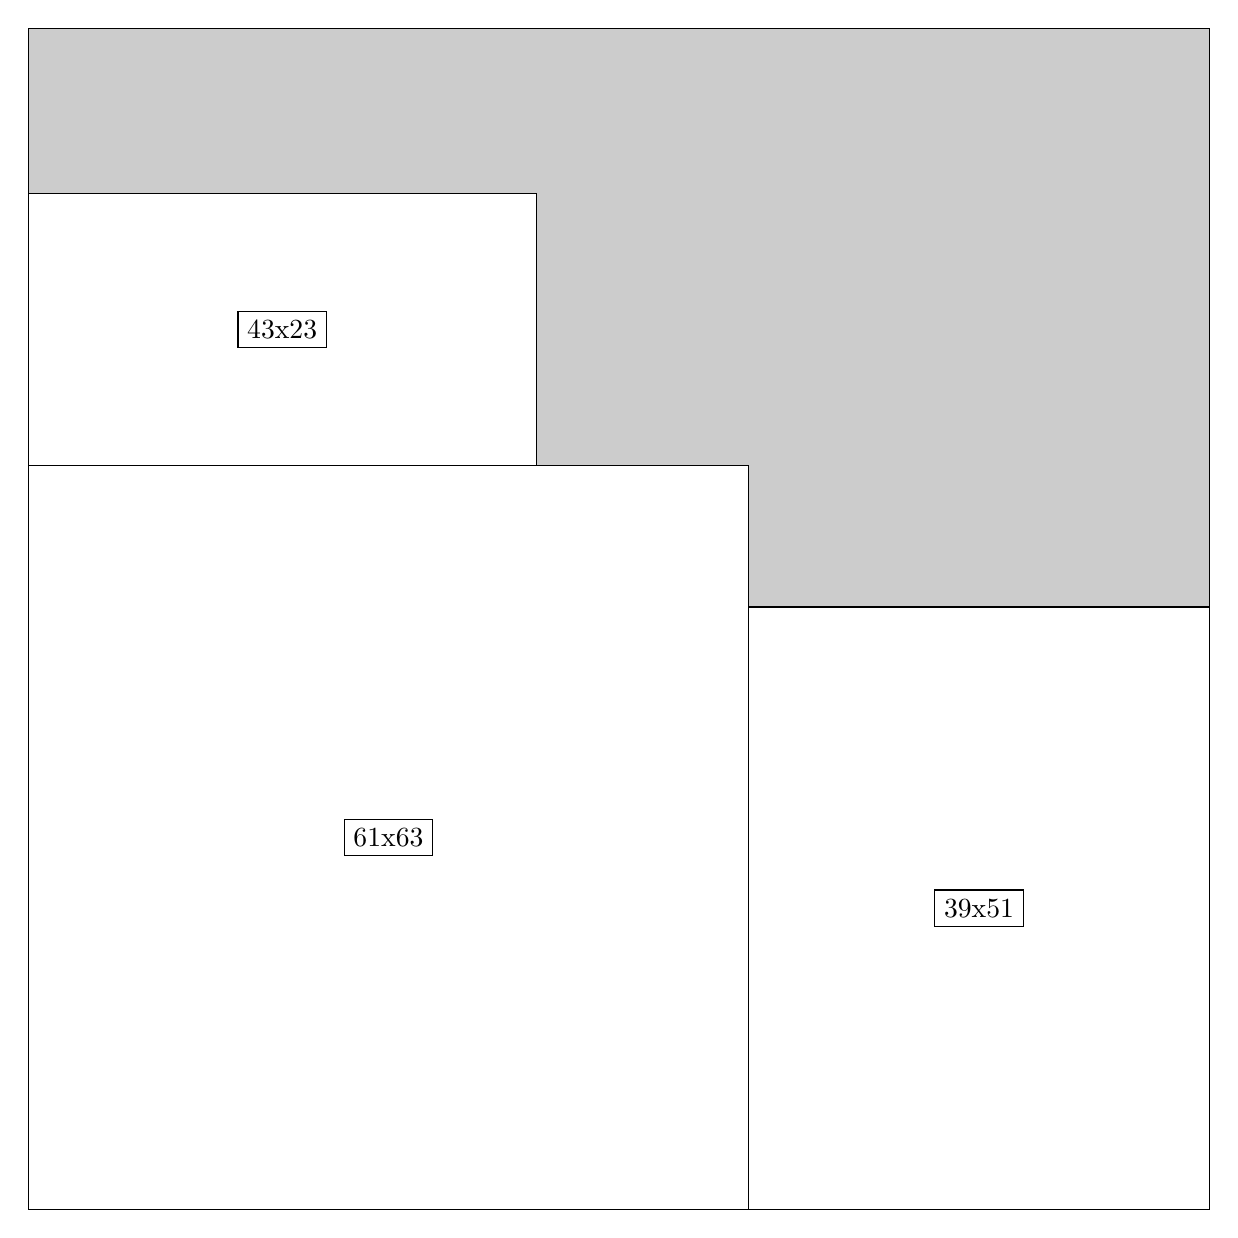
\begin{tikzpicture}[shorten >=1pt,scale=1.0,every node/.style={scale=1.0},->]
\tikzstyle{vertex}=[circle,fill=black!25,minimum size=14pt,inner sep=0pt]
\filldraw[fill=gray!40!white, draw=black] (0,0) rectangle (15.0,15.0);
\foreach \name/\x/\y/\w/\h in {61x63/0.0/0.0/9.15/9.45,39x51/9.15/0.0/5.85/7.6499999999999995,43x23/0.0/9.45/6.45/3.4499999999999997}
\filldraw[fill=white!40!white, draw=black] (\x,\y) rectangle node[draw] (\name) {\name} ++(\w,\h);
\end{tikzpicture}


w =61 , h =63 , x =0 , y =0 , v =3843
\par
w =39 , h =51 , x =61 , y =0 , v =1989
\par
w =43 , h =23 , x =0 , y =63 , v =989
\par
\newpage


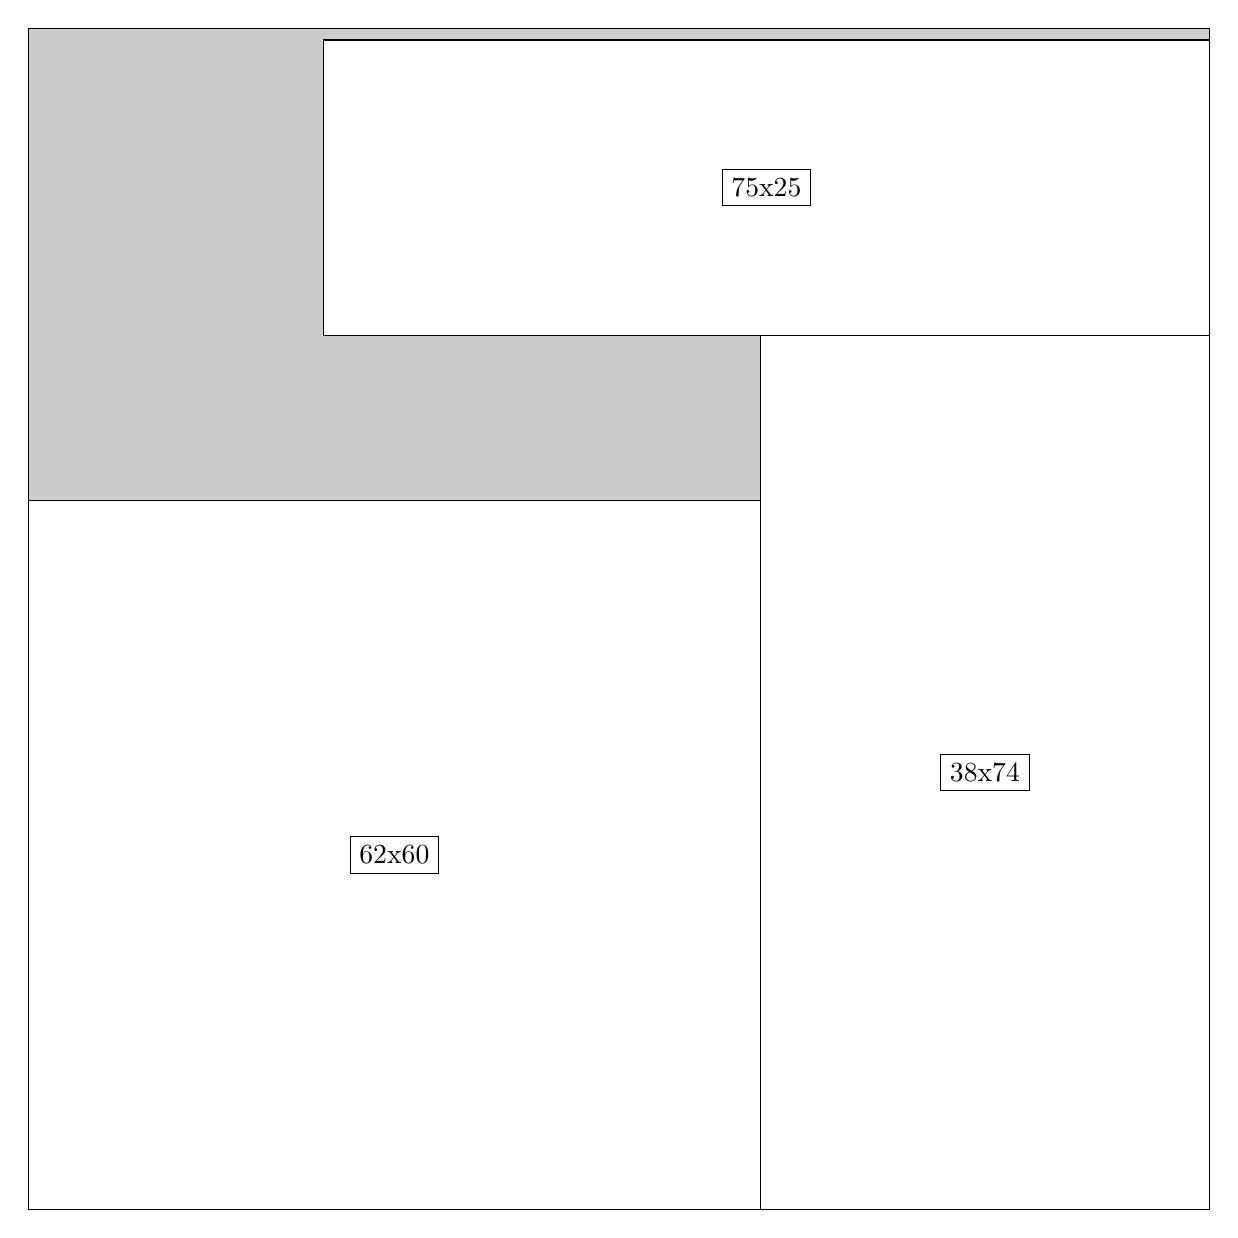
\begin{tikzpicture}[shorten >=1pt,scale=1.0,every node/.style={scale=1.0},->]
\tikzstyle{vertex}=[circle,fill=black!25,minimum size=14pt,inner sep=0pt]
\filldraw[fill=gray!40!white, draw=black] (0,0) rectangle (15.0,15.0);
\foreach \name/\x/\y/\w/\h in {62x60/0.0/0.0/9.299999999999999/9.0,38x74/9.299999999999999/0.0/5.7/11.1,75x25/3.75/11.1/11.25/3.75}
\filldraw[fill=white!40!white, draw=black] (\x,\y) rectangle node[draw] (\name) {\name} ++(\w,\h);
\end{tikzpicture}


w =62 , h =60 , x =0 , y =0 , v =3720
\par
w =38 , h =74 , x =62 , y =0 , v =2812
\par
w =75 , h =25 , x =25 , y =74 , v =1875
\par
\newpage


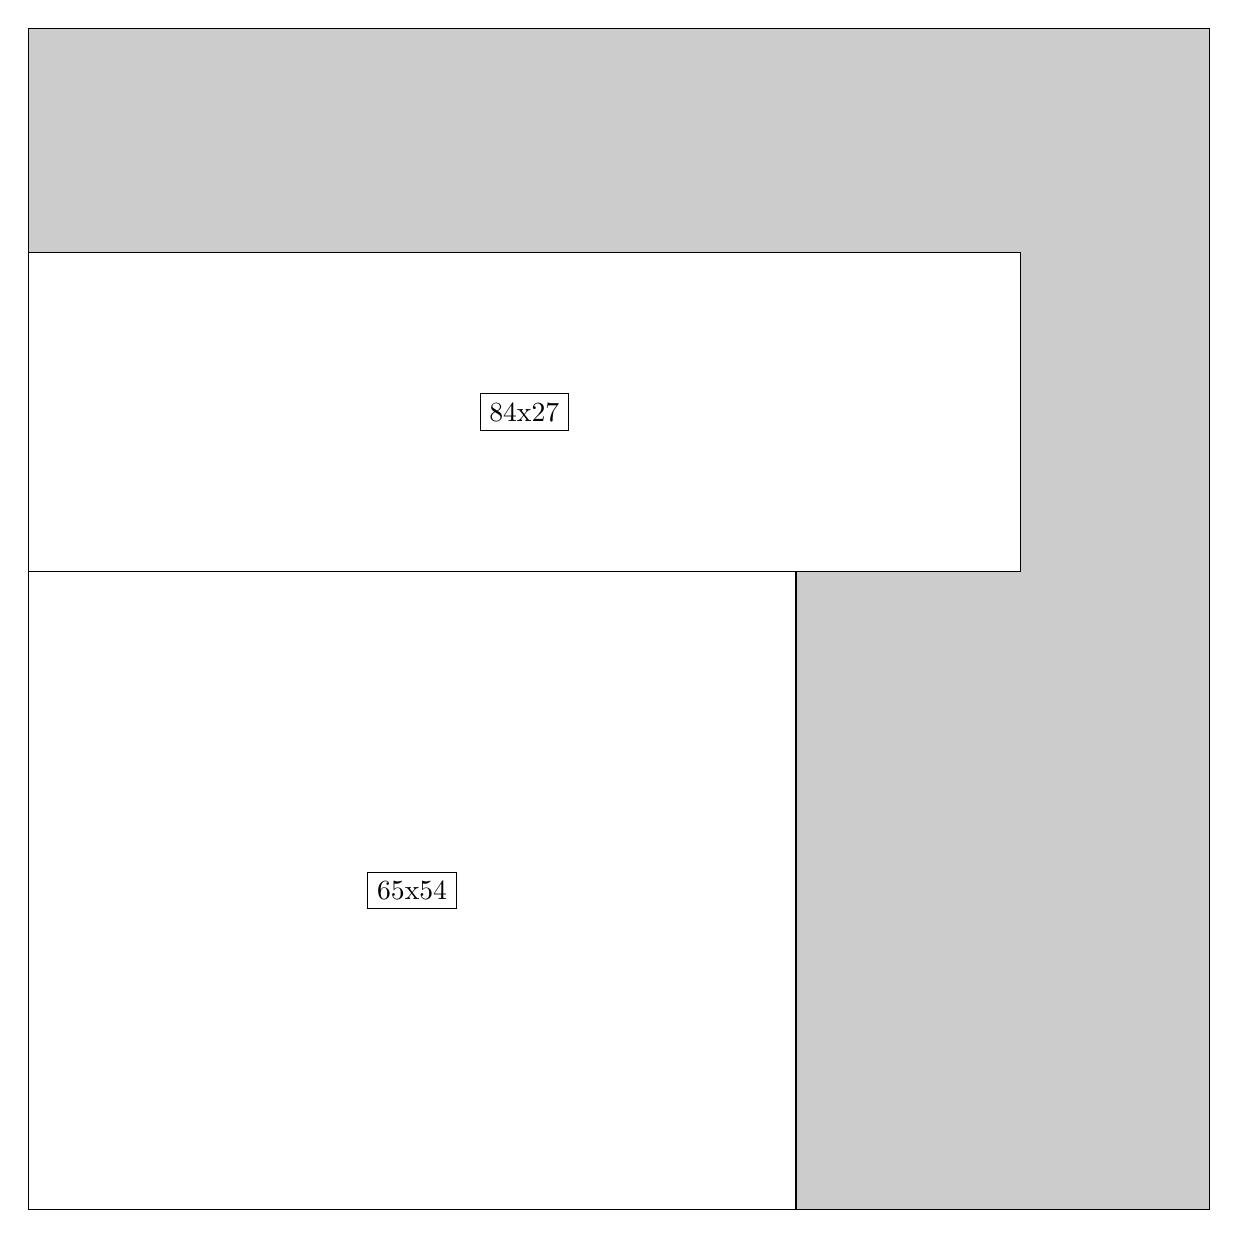
\begin{tikzpicture}[shorten >=1pt,scale=1.0,every node/.style={scale=1.0},->]
\tikzstyle{vertex}=[circle,fill=black!25,minimum size=14pt,inner sep=0pt]
\filldraw[fill=gray!40!white, draw=black] (0,0) rectangle (15.0,15.0);
\foreach \name/\x/\y/\w/\h in {65x54/0.0/0.0/9.75/8.1,84x27/0.0/8.1/12.6/4.05}
\filldraw[fill=white!40!white, draw=black] (\x,\y) rectangle node[draw] (\name) {\name} ++(\w,\h);
\end{tikzpicture}


w =65 , h =54 , x =0 , y =0 , v =3510
\par
w =84 , h =27 , x =0 , y =54 , v =2268
\par
\newpage


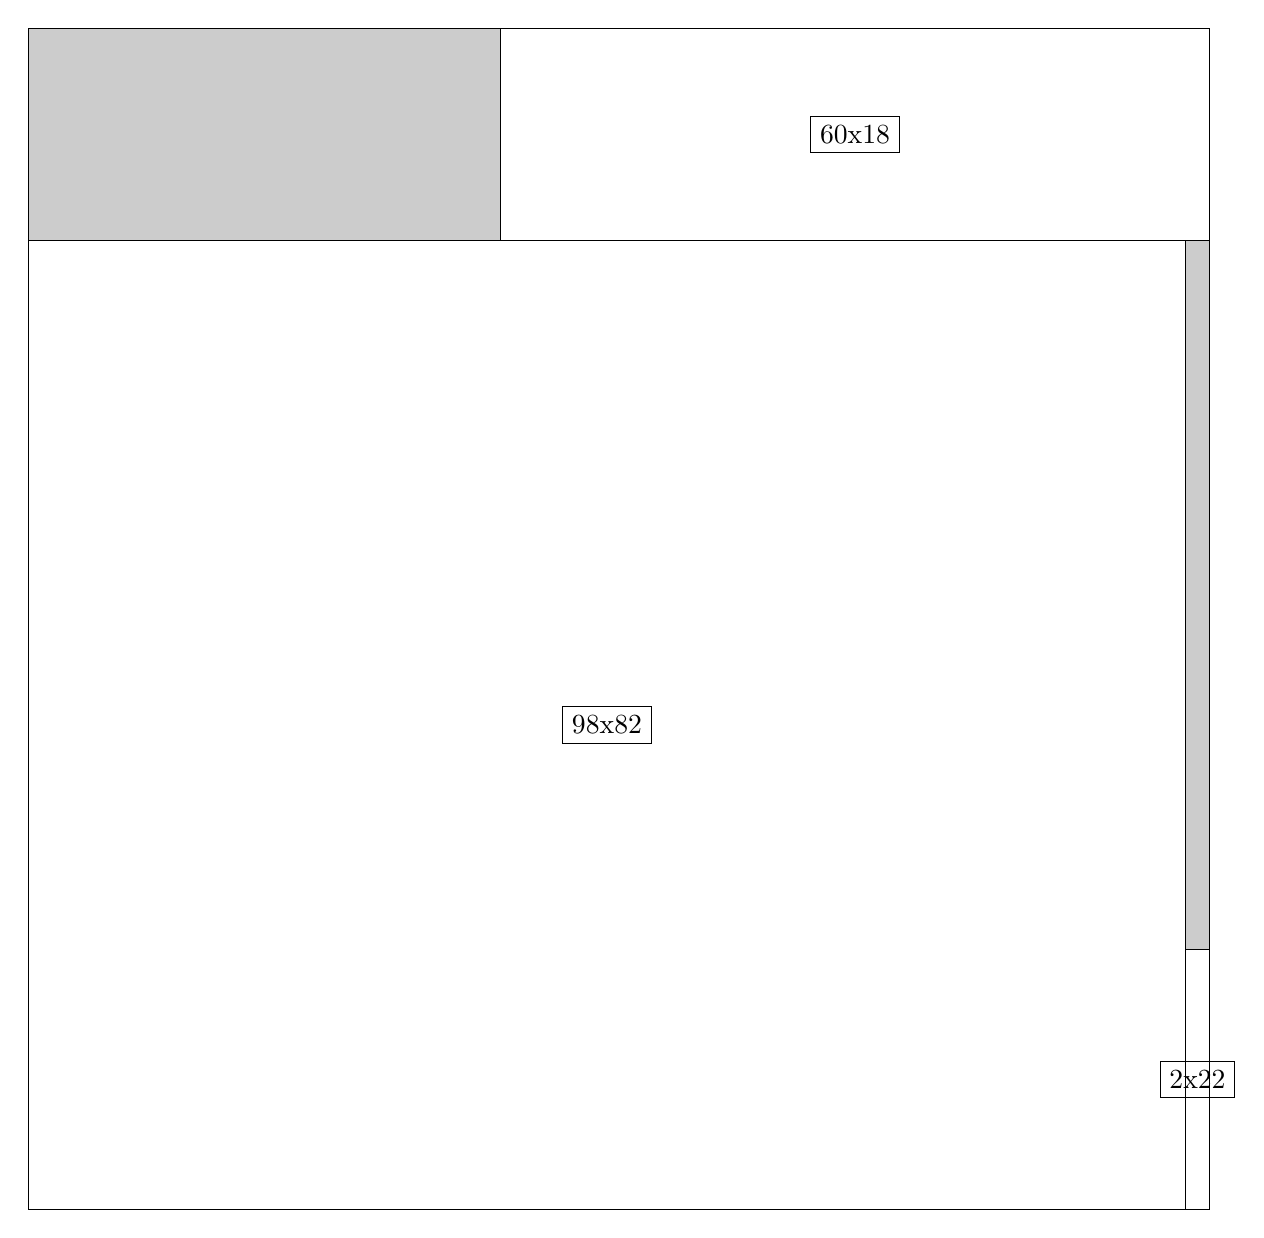
\begin{tikzpicture}[shorten >=1pt,scale=1.0,every node/.style={scale=1.0},->]
\tikzstyle{vertex}=[circle,fill=black!25,minimum size=14pt,inner sep=0pt]
\filldraw[fill=gray!40!white, draw=black] (0,0) rectangle (15.0,15.0);
\foreach \name/\x/\y/\w/\h in {98x82/0.0/0.0/14.7/12.299999999999999,60x18/6.0/12.299999999999999/9.0/2.6999999999999997,2x22/14.7/0.0/0.3/3.3}
\filldraw[fill=white!40!white, draw=black] (\x,\y) rectangle node[draw] (\name) {\name} ++(\w,\h);
\end{tikzpicture}


w =98 , h =82 , x =0 , y =0 , v =8036
\par
w =60 , h =18 , x =40 , y =82 , v =1080
\par
w =2 , h =22 , x =98 , y =0 , v =44
\par
\newpage


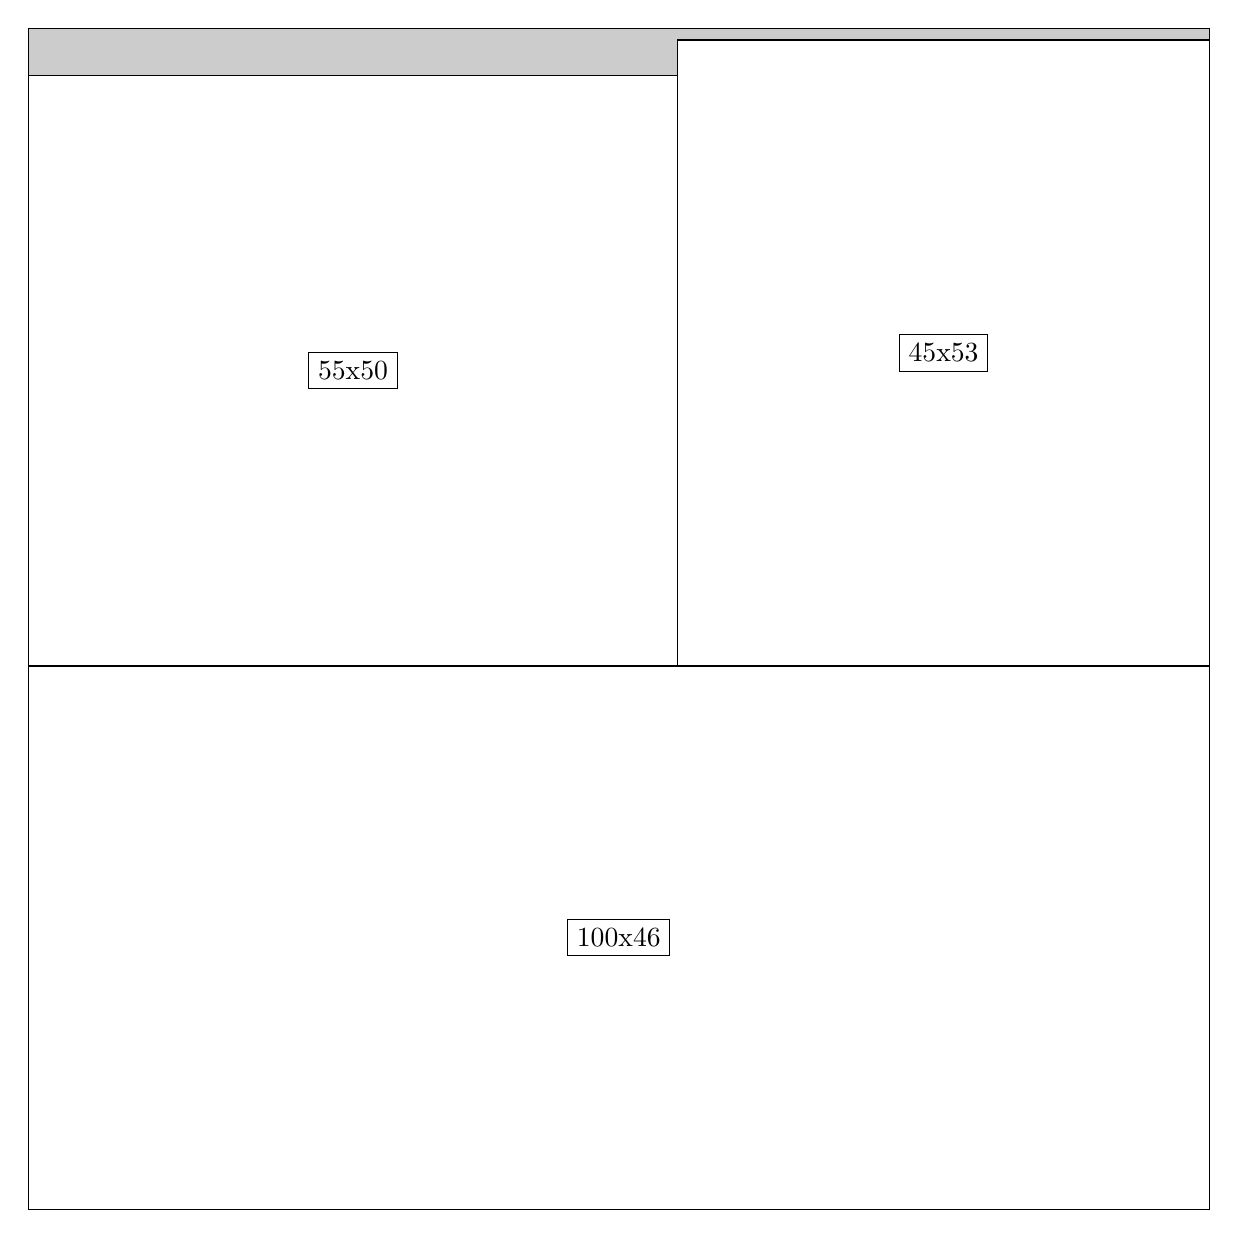
\begin{tikzpicture}[shorten >=1pt,scale=1.0,every node/.style={scale=1.0},->]
\tikzstyle{vertex}=[circle,fill=black!25,minimum size=14pt,inner sep=0pt]
\filldraw[fill=gray!40!white, draw=black] (0,0) rectangle (15.0,15.0);
\foreach \name/\x/\y/\w/\h in {55x50/0.0/6.8999999999999995/8.25/7.5,100x46/0.0/0.0/15.0/6.8999999999999995,45x53/8.25/6.8999999999999995/6.75/7.949999999999999}
\filldraw[fill=white!40!white, draw=black] (\x,\y) rectangle node[draw] (\name) {\name} ++(\w,\h);
\end{tikzpicture}


w =55 , h =50 , x =0 , y =46 , v =2750
\par
w =100 , h =46 , x =0 , y =0 , v =4600
\par
w =45 , h =53 , x =55 , y =46 , v =2385
\par
\newpage


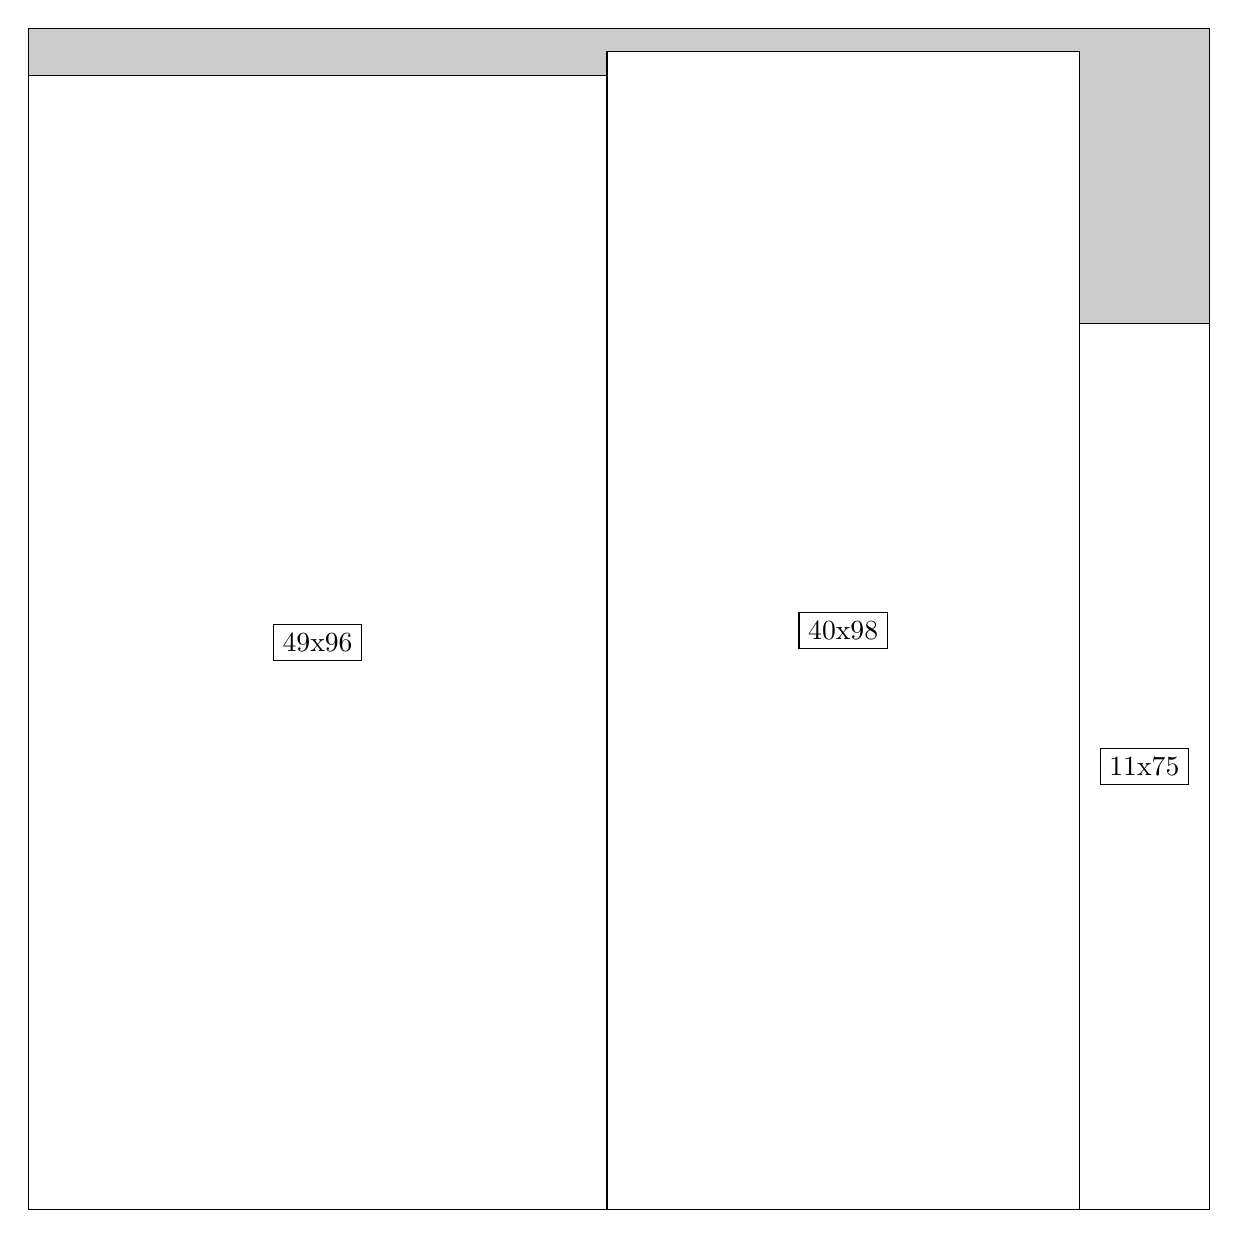
\begin{tikzpicture}[shorten >=1pt,scale=1.0,every node/.style={scale=1.0},->]
\tikzstyle{vertex}=[circle,fill=black!25,minimum size=14pt,inner sep=0pt]
\filldraw[fill=gray!40!white, draw=black] (0,0) rectangle (15.0,15.0);
\foreach \name/\x/\y/\w/\h in {49x96/0.0/0.0/7.35/14.399999999999999,40x98/7.35/0.0/6.0/14.7,11x75/13.35/0.0/1.65/11.25}
\filldraw[fill=white!40!white, draw=black] (\x,\y) rectangle node[draw] (\name) {\name} ++(\w,\h);
\end{tikzpicture}


w =49 , h =96 , x =0 , y =0 , v =4704
\par
w =40 , h =98 , x =49 , y =0 , v =3920
\par
w =11 , h =75 , x =89 , y =0 , v =825
\par
\newpage


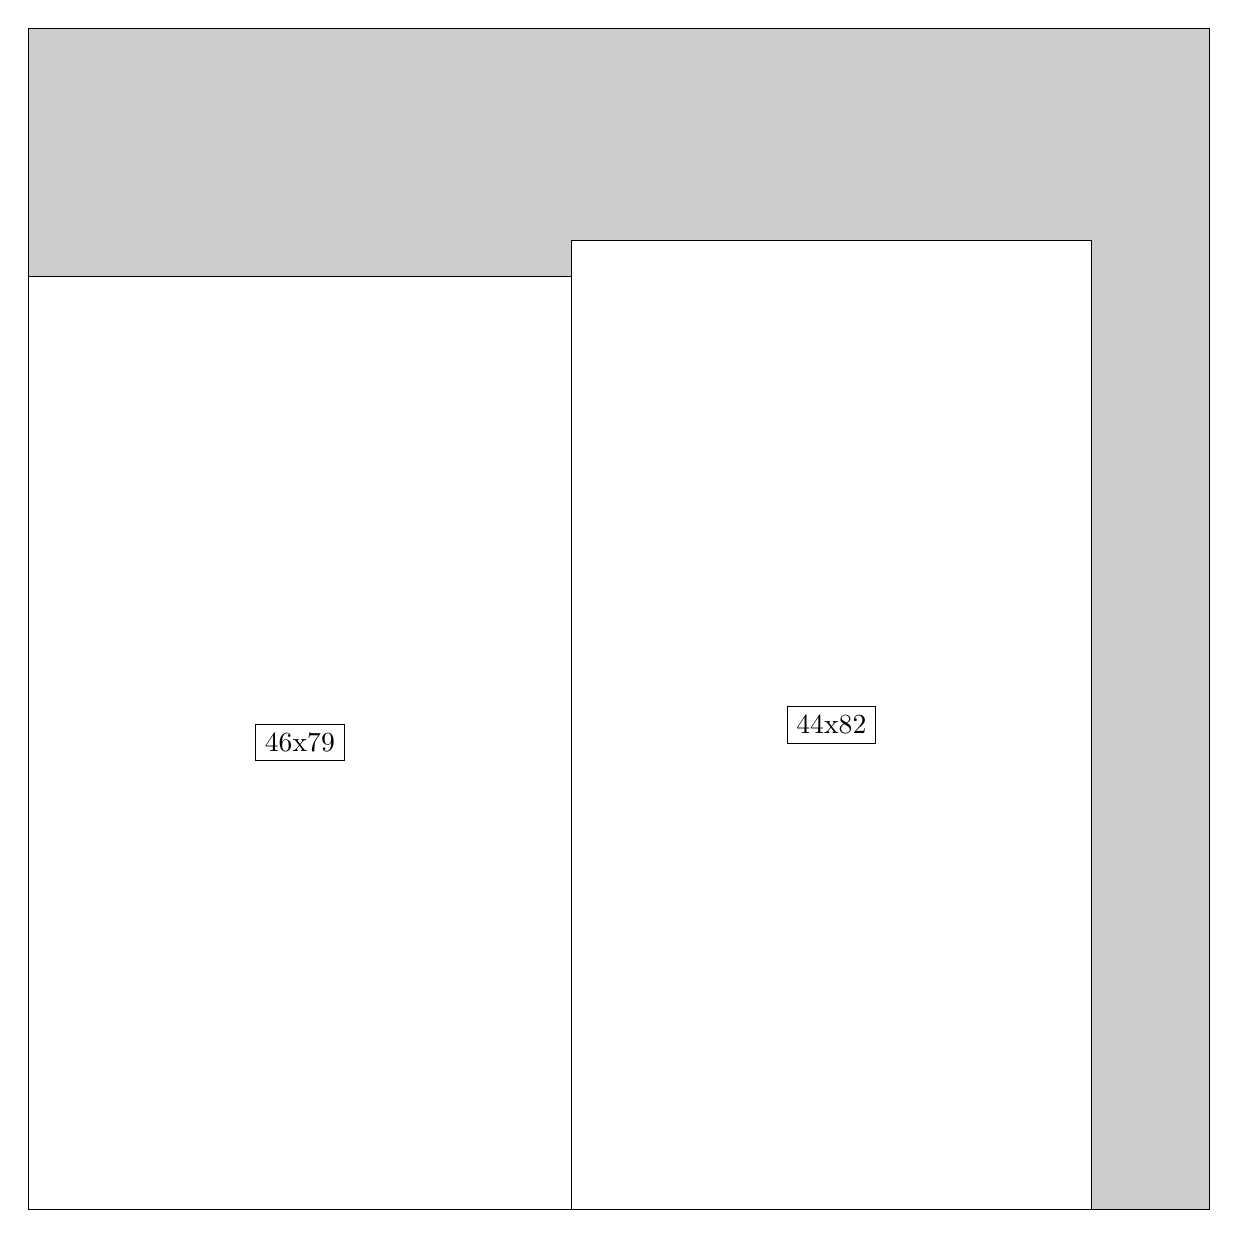
\begin{tikzpicture}[shorten >=1pt,scale=1.0,every node/.style={scale=1.0},->]
\tikzstyle{vertex}=[circle,fill=black!25,minimum size=14pt,inner sep=0pt]
\filldraw[fill=gray!40!white, draw=black] (0,0) rectangle (15.0,15.0);
\foreach \name/\x/\y/\w/\h in {46x79/0.0/0.0/6.8999999999999995/11.85,44x82/6.8999999999999995/0.0/6.6/12.299999999999999}
\filldraw[fill=white!40!white, draw=black] (\x,\y) rectangle node[draw] (\name) {\name} ++(\w,\h);
\end{tikzpicture}


w =46 , h =79 , x =0 , y =0 , v =3634
\par
w =44 , h =82 , x =46 , y =0 , v =3608
\par
\newpage


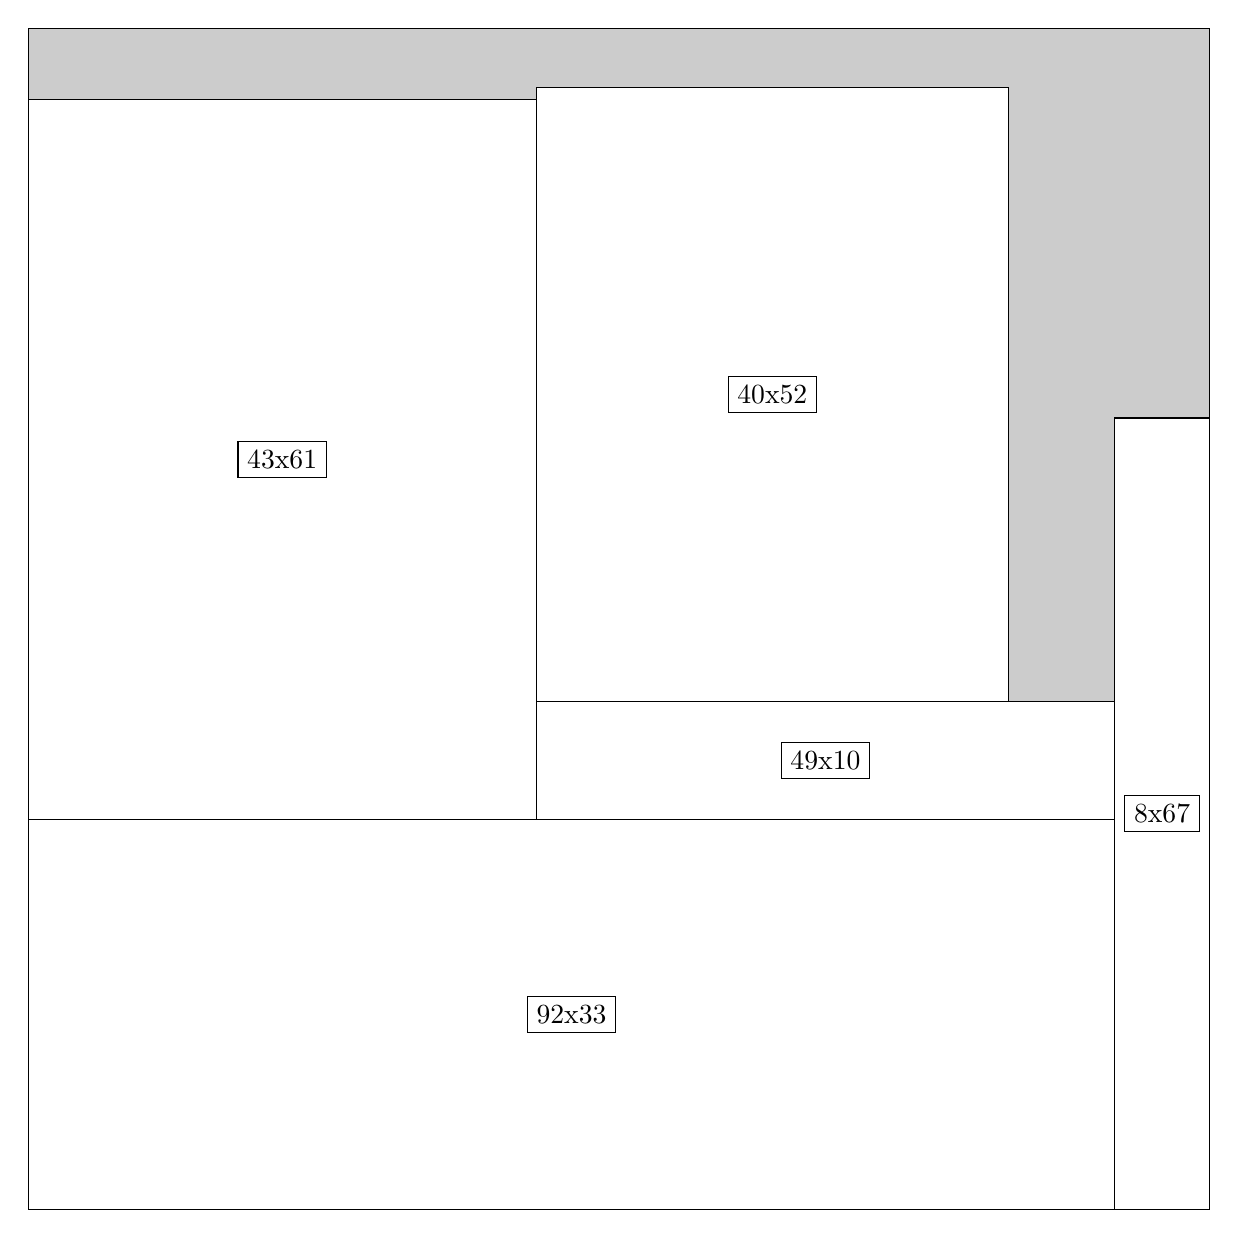
\begin{tikzpicture}[shorten >=1pt,scale=1.0,every node/.style={scale=1.0},->]
\tikzstyle{vertex}=[circle,fill=black!25,minimum size=14pt,inner sep=0pt]
\filldraw[fill=gray!40!white, draw=black] (0,0) rectangle (15.0,15.0);
\foreach \name/\x/\y/\w/\h in {92x33/0.0/0.0/13.799999999999999/4.95,43x61/0.0/4.95/6.45/9.15,40x52/6.45/6.45/6.0/7.8,8x67/13.799999999999999/0.0/1.2/10.049999999999999,49x10/6.45/4.95/7.35/1.5}
\filldraw[fill=white!40!white, draw=black] (\x,\y) rectangle node[draw] (\name) {\name} ++(\w,\h);
\end{tikzpicture}


w =92 , h =33 , x =0 , y =0 , v =3036
\par
w =43 , h =61 , x =0 , y =33 , v =2623
\par
w =40 , h =52 , x =43 , y =43 , v =2080
\par
w =8 , h =67 , x =92 , y =0 , v =536
\par
w =49 , h =10 , x =43 , y =33 , v =490
\par
\newpage


\end{document}